\documentclass[a4paper,12pt]{article}
\usepackage[left=3cm,right=2.5cm,top=2.5cm, bottom=2.5cm]{geometry} 
\usepackage[utf8]{inputenc}
\usepackage{t1enc}
\usepackage{graphicx}
\usepackage[magyar]{babel}
\usepackage[nottoc]{tocbibind}%hogy az irodalomjegyzék is benne legyen a tartalomjegyzékben
\usepackage{pdfpages}

\usepackage{commath} %abszolút érték jelhez.
\usepackage{multirow}
\usepackage{subcaption}
\usepackage{subfig}



%matgót megoldottam a 2. sorban.
%\usepackage{anysize} %margóhoz
%\marginsize{3cm}{3cm}{2.5cm}{2.5cm}


%ha esetleg ki akarod szerni az összes ábrát ->
%\usepackage{comment}
%\excludecomment{textcolor}
%\excludecomment{figure}
%\let\endfigure\relax
%<-
\linespread{1.3} %1.3 = másfélszeres sorköz.
%\usepackage{showframe} -> megjelnnek a margók.

\begin{document}
\frenchspacing
%%%%%%%%%%%%%%%%%%%%%%%%%%%%%%%%%%%%%%%%%%%%%%%%%%%%%%%%%%%%%%%%%


\pagenumbering{gobble}

 \begin{center} 
\includegraphics[width=80mm,keepaspectratio]{abrak/bmelogo.jpg}\\ \vspace{0.3cm}  \Large Diplomamunka \\[1.5cm] \vspace{0.5cm} { \large \textbf{ Mikro-CT készülék rekonstrukciós és kalibrációs környezetének létrehozása}}\\[2.5cm] \vspace{0.2cm} \large Marinovszki Árpád\\[5cm] \begin{tabular}{ll} Témavezető: & Dr.\ Légrády Dávid \\ & egyetemi docens \\ & BME Nukleáris technika Intézet \\ \end{tabular} \vfill \large BME \\ \large 2016 \end{center} 
 
 \clearpage \setcounter{page}{1}
 \pagenumbering{arabic}
 
   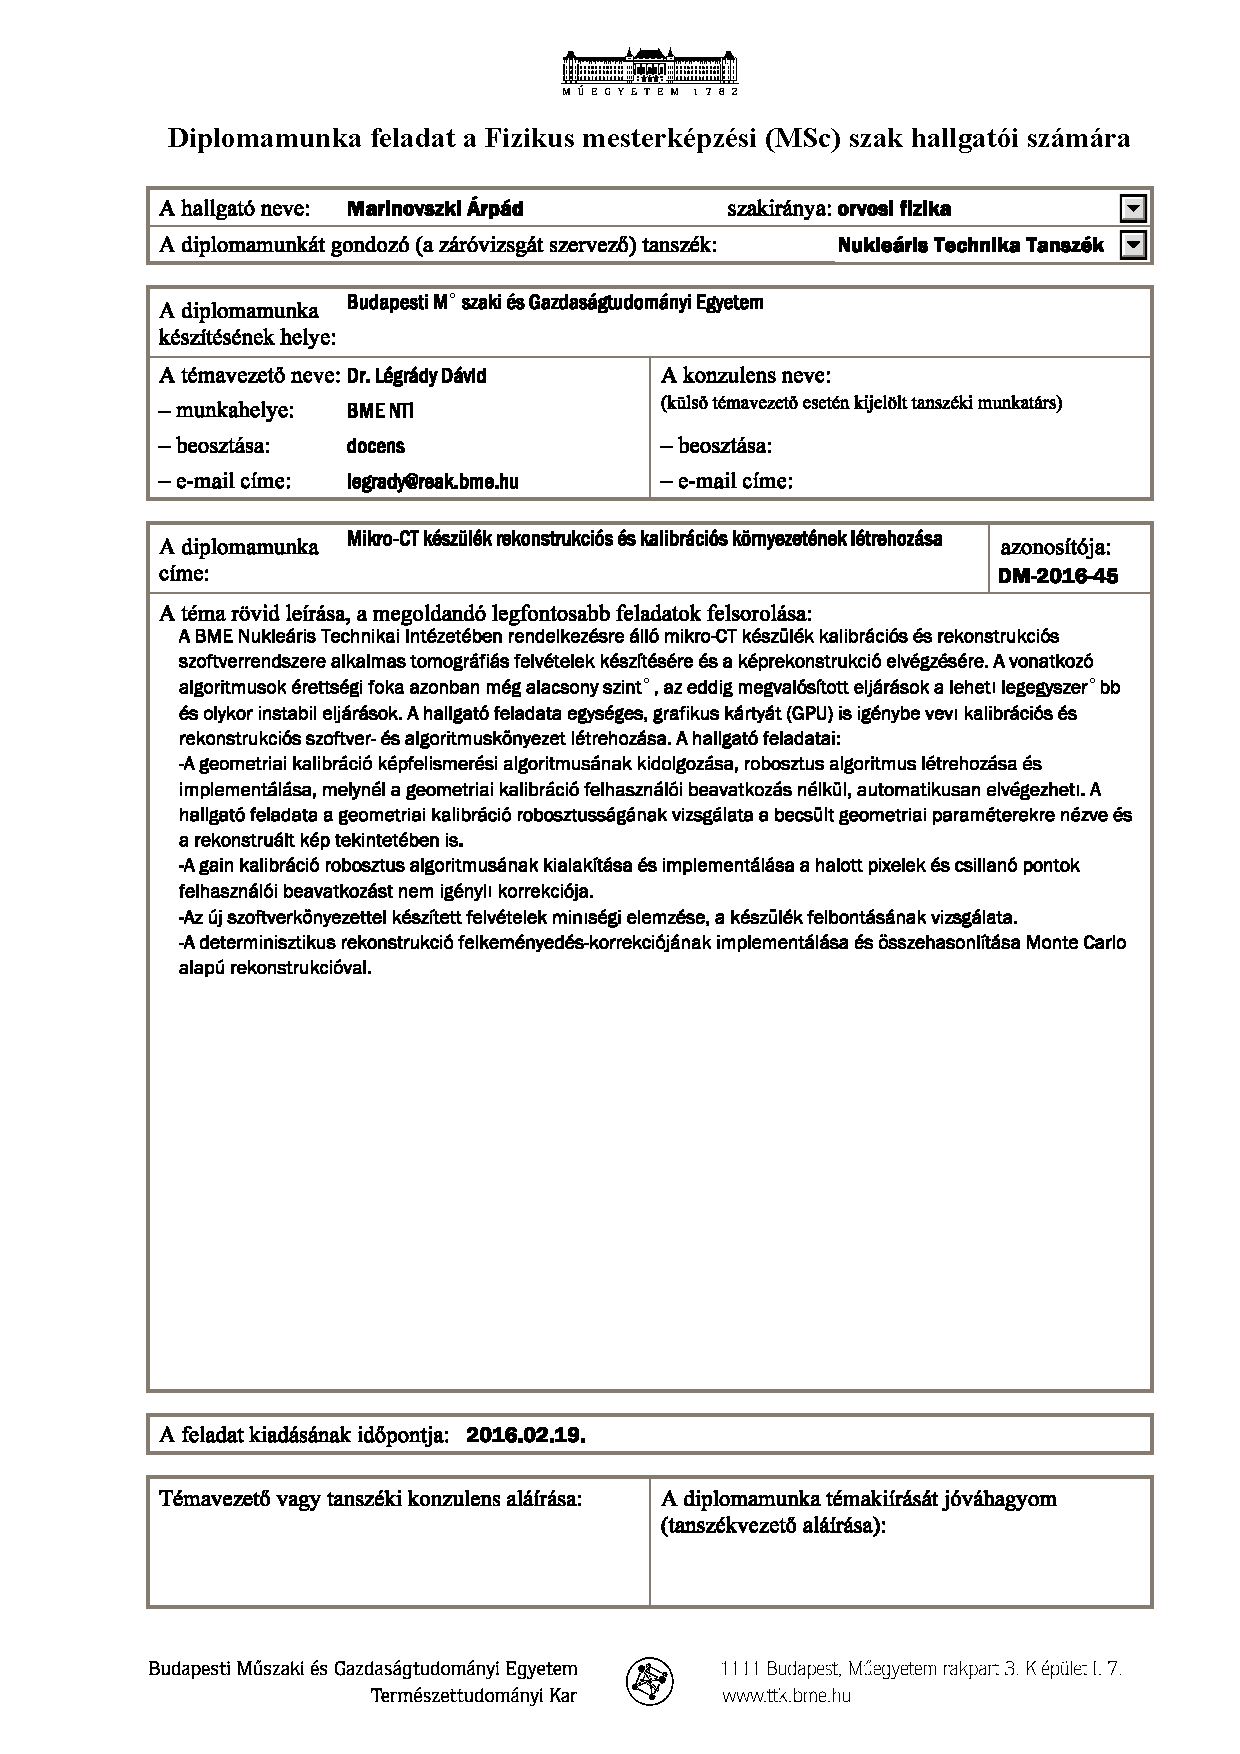
\includepdf[ pagecommand={}]{abrak/jelentkezes.pdf}

\clearpage

{\large Önállósági nyilatkozat}
\\[0.5cm]



Alulírott Marinovszki Árpád a Budapesti Műszaki és Gazdaságtudományi Egyetem fizikus MSc szakos hallgatója kijelentem, hogy ezt a diplomamunkát meg nem engedett segédeszközök nélkül, önállóan, a témavezető irányításával készítettem, és csak a megadott forrásokat használtam fel. 


Minden olyan részt, melyet szó szerint, vagy azonos értelemben, de átfogalmazva más forrásból vettem, a forrás megadásával jelöltem.
\\[0.3cm]

Budapest, 2016.\ június 6.

\hspace{9cm}\makebox[1.5in]{\hrulefill}

\hspace{9cm}\makebox[1.5in]{\centering aláírás}




\clearpage


 \tableofcontents

\clearpage

	






%CSAPJUNK A LECSÓBA
%TODO majd egyeztesd az egyes fejezeteken belül a személyeket és az igeidőt (csináljuk / csinálják/ csinálták stb)
%BEVEZETÉS------------------------------------------------------
\section{Bevezetés}


A CT, avagy Computed Tomograpgy -- magyarul komputertomográfia vagy számítógépes tomográfia -- a modern orvosi képalkotó eljárások  aktívan kutatott, esetenként megkerülhetetlen eszköze, amely a vizsgált páciens testének belső szerkezetéről ad információt. Az orvosi alkalmazások mellett  gyakran használják a technikát állatok vizsgálatához, valamint élettelen tárgyak roncsolásmentes vizsgálatához is. A BME Nukleáris Technika Intézetében 2013--2014 között került sor egy kis méretű kúpsugaras -- ún.~ Cone-Beam, vagy röviden CB-- CT berendezés beüzemelésére, a hallgatók aktív közreműködése mellett. Jelen diplomamunkában ezt a munkafolyamatot folytatva tökéletesítem a megalkotott eszközöket, illetve dolgozok ki új metódusokat az eddig nem orvosolt problémák megoldására. Diplomamunkám elején röviden összefoglalom a CT működési hátterét, ismertetem a tanszéken rendelkezésre álló eszközöket és a rendszer eddig megtervezett részeit. Ez után összegzem a jelen diplomamunkában kitűzött feladatokat és ismertetem a megvalósításukhoz használt eszközöket.

\subsection{A Cone-Beam CT működése } 


A  CT felvételek elkészítésekor röntgensugárzással világítjuk át a vizsgált objektumot, hogy információt szerezzünk annak belső szerkezetéről. A Cone-Beam jelző arra utal, hogy a pontszerű röntgenforrás mellett síkdetektort használunk, így a detektált nyaláb kúp alakú. Egy ilyen elrendezés vázlatos rajza látható \aref{fig:cbct}.~ábrán.  A teljes vizsgálat során a detektort és a forrást $360^\circ$-ban körbeforgatják a vizsgált objektum körül, vagy, mint ahogy az általunk használt berendezésnél történik, az objektumot forgatják körbe, miközben a többi berendezés nem mozdul. A detektorból kiolvasott képeket hívjuk az adott elfordulás mellett kapott projekciónak. Ezen képen a kibocsátott sugárzás azon hányadával arányos intenzitásérték jelenik meg, amely hányad az objektumban nem nyelődött el. Az objektum elnyelési képességét jellemző $\mu(\underline{r})$ helyfüggő lineáris gyengítési együttható segítségével a detektort érő sugárzás $I$ intenzitása felírható a Beer-Lambert (\ref{eq:BL}) törvény segítségével, ahol $I_0$ jelöli a röntgenforrásból az adott pixel térszögébe irányuló sugárzás intenzitását, az integrálás pedig a forrást a detektor adott pixelével összekötő $L$ egyenes mentén történik. A képletben, és az analitikus Cone-Beam rekonstrukció során általában, elhanyagolásra kerül többek között a gyengítési együttható és a sugárzás intenzitásának energiafüggése, valamint a különböző szórási folyamatok.  


\begin{figure}[htbp]
\center
\includegraphics[width=0.6\textwidth]{abrak/cbct}
\caption{A Cone-Beam CT vázlatos rajza\cite{noo}.}
\label{fig:cbct}
\end{figure}



\begin{equation}
\label{eq:BL}
I=I_0 \cdot e^{-\int_L \mu(\underline{r}) d\underline{r}}
\end{equation}


Mivel a gyengülés nélkül kapott $I_0$ intenzitás meghatározható, az átvilágítás során fizikai információt a fenti egyenlet átrendezéséből  kapható (\ref{eq:BLmu}) kifejezés adja, amely az objektum lineáris gyengítési együtthatója egy adott egyenes mentén integrálva.



\begin{equation}
\label{eq:BLmu}
{\int_L \mu(\underline{r}) d\underline{r}} = -\ln \left(\frac{I}{I_0} \right)
\end{equation}

A CT vizsgálat feladata a gyengítési együttható különböző egyenesek mentén integrált értékeiből visszaállítani annak 3 dimenziós eloszlását. Ezt a lépést visszavetítésnek hívjuk, és megvalósítása a projekciók inverz Radon-transzformálásával történik. 

\subsection{A tanszéken rendelkezésre álló eszközök}

Az egyetem reaktorépületében beüzemelt CT képalkotó berendezés a következő elemekből áll. 
\begin{itemize}
\item Röntgenforrásként egy \emph{Source Ray SB-80-1k}  típusú mikrofókuszos röntgencsövet használunk, amely kis méretű fókuszfolttal ( min.\ $33\mu \text m$) rendelkezik, $35$--$80$~kV közötti gyorsítófeszültséggel és $20$--$1000$~mA közötti áramerősséggel üzemeltethető.  
\item Detektorként egy \emph{Dexela 1207}  síkdetektort használunk, amely $114,\!9$ x $64,\!6~\text{mm}^2$ érzékeny felülettel rendelkezik, amellyel $12$--$130$~kV közötti Röntgen-energiákra érzékeny. Pixeleinek élhossza $74,\!8~\mu\text{m}$, így a felbontása $1536 x 864$~pixel.  
\item A vizsgált objektum forgatásáért egy \emph{PHI Instruments} gyártmányú rotációs asztal felel, amelyet két \emph{RDM 564/50, BERGER LAHR} típusú léptetőmotor hajt, minimálisan  $0,\!72^\circ$-os lépésközzel.
\end{itemize}


A rendszer által leképezhető objektum nagyságát a detektor méretei behatárolják, hiszen az objektum képe teljes szélességében a detektorra kell, hogy essen. Így maximálisan $\approx10~\text{cm}$ átmérőjű tárgyak vizsgálhatók a berendezéssel. Az egyes elemek azonban nincsenek egymáshoz képest fixen rögzítve, azok szabadon mozgathatóak, így kisebb objektumokról is megfelelő minőségű felvételeket tudunk készíteni: minél közelebb helyezzük a tárgyat a forráshoz, annál inkább nagyított képet kapunk a detektoron. Éppen az efféle átrendezhetőség miatt fontos elvárás, hogy a geometria adatait rutinszerűen, gyorsan és pontosan lehessen meghatározni, hiszen a visszavetítéshez szükséges ezen adatok pontos ismerete. Ezt a műveletet, azaz a tárgy forgástengelyének, a forrásnak és a detektornak az egymástól való távolságának a meghatározását nevezzük geometriai kalibrációnak, amelyről részletesen \aref{sec:geomkalib}.~fejezetben írok.

\subsection{A CT vizsgálathoz rendelkezésre álló szoftverek}


A teljes rendszer összeszerelése és a szükséges szoftverek megalkotása is  korábbi hallgatók által lett kivitelezve. Így rendelkezésre áll egy \emph{C\#} nyelven írt, grafikus felülettel rendelkező mérésvezérlő szoftver, amely Kleizer Gábor készített, részben korábbi szagdolgozata\cite{kleizer} alapján. Ez a szoftver felelős a röntgencső vezérléséért és az ehhez kapcsolódó biztonsági berendezések működtetéséért (fényjelzés a röntgencső működése közben, stb.). Ugyancsak ez a szoftver vezérli a tárgy forgatásáért felelős léptetőmotorokat, és kommunikál a detektorral. A szoftver tehát teljes körűen elvégez minden, a CT felvételek elkészítéséhez szükséges feladatot, a képeket pedig bináris formátumban a merevlemezre menti. Az elkészült képekről tudni érdemes, hogy a pixelek értékei $0$ és $  \left ( 2^{14}-1 \right ) = 16~383$ közötti egész számot vehetnek fel, amely szám a detektor adott pixelére eső sugárzás intenzitásával arányos a detektor mérési tartományában.


A képek feldolgozására két, az előbbitől és egymástól is független szoftver áll rendelkezésre. A vizsgált tárgy 3 dimenziós képének visszaállításáért felelős szoftvert Deli Gábor\cite{deli} írta meg, diplomamunkája során. Ez a program \emph{C++} és \emph{CUDA} nyelven íródott. Utóbbi egy olyan platformot nyújt, amely segítségével a visszavetítésért felelős képműveletek párhuzamosan és igen gyorsan végezhetők el. Erről  \aref{sec:cuda}.~fejezeten írok részletesen. 


Másrészt a geometriai kalibráció elvégzéséért, valamint a detektorpixelek eltérő tulajdonságaiból származó képhibák eltüntetéséért felel a Tölgyesi Botond által, diplomamunkája \cite{botond} keretei közt készített szoftver. A \emph{MATLAB} nyelven íródott program  képes \aref{sec:gainkorr}.~fejezetben bemutatott gain hibák kezelésére, valamint \aref{sec:geomkalib} .~fejezetben részletezett geometriai kalibráció elvégzésére is. Ezeket a funkciókat azonban viszonylag lassan végzi el, erőforrásigénye igen nagy (akár $10$--$20$~GB RAM). Ezen kívül a képfeldolgozás során alkalmazott módszerei nem a leghatásosabbak, eredményességük nagyban függ  a felhasználó által megadott paraméterektől és a kalibrációs adatsor minőségétől. Ugyanakkor Tölgyesi megmutatta, hogy optimális körülmények között a szoftver képes a feladatok jó minőségű elvégzésére. A képek gain korrigálás igen jó minőségben képes kivitelezni, és megfelelő paraméterek megválasztásával a geometriai kalibrációs is helyes eredményt szolgáltat. Az alkalmazott algoritmusai tehát alapvetően helyesek, amelyeket Tölgyesi részletes tesztekkel is alátámasztott. Diplomamunkámban ezeket a  funkciókat fejlesztettem tovább,  hogy azok gyorsan, hatékonyan  és pontosan legyenek képesek feladatuk elvégzésére. A részben instabil működése miatt  a korábban  megvalósított szoftverre, illetve annak algoritmusara a továbbiakban \emph{kísérleti algoritmus}ként hivatkozom.



\section{Célkitűzés}


Jelen diplomamunkámban a Tölgyesi Botond által vizsgált gain korrekciós és geometria kalibrációs módszereket ültetem át \emph{MATLAB} környezetből grafikus felülettel rendelkező, felhasználóbarát környezetbe. A feladat elvégzése során szem előtt tartva, hogy a megvalósított funkciók minél gyorsabban, alacsony erőforrást igényelve, a felhasználó által a lehető legkevesebb beavatkozást igényelve fussanak le. Ennek érdekében a képek feldolgozását \emph{CUDA} nyelven valósítom meg, az elkészítendő program pedig \emph{Qt} grafikus felületet kap. A geometriai kalibráció esetében új képfeldolgozási algoritmust vezetek be, amelyek pontosabb eredményt szolgáltat, mint az eddigiekben megvalósított. Ezen kívül a geometriai kalibrációs adatok meghatározásánál számolom és számon tartom a kalibrációs mérések hibáit. A hibákat figyelembe veszem a geometriai adatok számolásánál, így a képek feldolgozása során vétett pontatlanságokat a szoftver a felhasználó beavatkozása nélkül kezeli.


Az új algoritmusok, illetve megvalósításuk helyességét a CT-vel készült képek alapján tesztelem. Ilyen képekből azonban  viszonylag kevés áll rendelkezésre, mivel jelen diplomamunkát az ajánlott félév utáni félévben kezdtem el. A megfelelő minőségű képek gyártását tovább nehezítette, hogy a reaktor épületét időközben felújítás miatt lezárták, így az ott összeszerelt CT berendezés is hozzáférhetetlenné vált. A felvételek elkészítésére így limitált idő állt rendelkezésemre. Emiatt megfelelő minőségű geometriai kalibrációs felvételekből csak egy széria áll rendelkezésemre, az eredményeimet ennek használatával fogom bemutatni.





\section{Az alkalmazott szoftveres megoldások}

\subsection{CUDA}
\label{sec:cuda}


A \emph{CUDA} programnyelv az \emph{NVIDIA} nevű, grafikus kártyákat fejlesztő cég saját, \emph{C++}-hoz hasonló szerkezetű programnyelve, amellyel az általuk megalkotott videokártyákon lehet általános célú, párhuzamos programozást igénylő feladatokat megvalósítani. A képfeldolgozásban általában igen sok művelet alkalmas a párhuzamosításra, ezért is alkalmazzák előszeretettel ezen a területen is. A képműveletek gyors elvégzése érdekében én is \emph{CUDA} nyelven írtam meg a képek feldolgozását végző kódrészleteket. 


A grafikus kártyán való párhuzamos feldolgozást illetően elmondható, hogy egy adott munkafolyamat több szinten szerveződő struktúrába foglalható.  A legalacsonyabb szintű működésért az ún.\ \emph{thread}-ek, vagyis \emph{szálak} felelnek, amik a tulajdonképpeni utasításokat végrehajtó egységek. Ezeknek saját, gyors elérésű, de limitált mennyiségű memória áll rendelkezésre. A thread-ek \emph{blokkokba} csoportosíthatók. Az egy blokkon belüli szálak egymással kommunikálhatnak, a blokk minden szála által használható, közepes sebességű \emph{megosztott}, vagyis úgynevezett \emph{shared} memória segítségével. Míg a szálak saját memóriája, illetve a blokkon belüli shared memória csak ideiglenes tárolóként szolgál, a videókártya \emph{globális} memóriájában lehet a különböző műveletek között eltárolni a feldolgozandó adatokat. Szintén a globális memória szolgál a számítógép virtuális, ún.\ \emph{host} memóriájával. A globális memória mérete általában igen nagy, elérési sebessége viszont az előbb említett alacsonyabb szintű memóriaterületekhez képest lassú. A memóriaterületek ilyen szintű szerveződése igen sok lehetőséget ad a \emph{CUDA} programok futási sebességének további optimalizációjához.

A nyelv további tulajdonsága, hogy a megírt programkód sebessége skálázódik a számítógépben lévő grafikus kártya sebességével. Vagyis ugyan az a programkód minden féle módosítás nélkül is gyorsabban fut egy nagyobb teljesítményű grafikus kártyán. Ez viszont némi megkötésekkel jár, így a \emph{CUDA} programok futtatásakor a rendszer a következő garanciákat teszi. Egy adott párhuzamos feladat, vagyis \emph{kernel} futtatása során a szálak 32 elemű csoportokban, úgynevezett \emph{warp}-okban futnak. Egy warp-on belül minden szál pontosan ugyan azt a műveletet hajtja végre, párhuzamosan. A kernelnek megadhatjuk, hogy hány blokkot, és azokon belül hány szálat indítson az adott feladat elvégzéséhez, de nincs garancia arra, hogy ezek milyen sorrendben fognak lefutni. Ezek kissé laza feltételeknek látszanak, amiket a program tervezése során valóban szem előtt kell tartani, azonban így megoldható az, hogy egyszerre annyi párhuzamos szálon fusson a kívánt művelet, amennyi rendelkezésre áll.

\subsection{Qt}

A reaktor lezárása miatt elszállításra került a mérésvezérlő, nagy teljesítményű  számítógép is, amelyen a jövőben futtatni szeretnénk az általam megalkotott szoftvert.  Ezen a számítógépen Windows operációs rendszer fut, minthogy a mérésvezérlő szoftver csak ilyen platformra lett megírva. A kísérleti algoritmussal való összehasonlításhoz azonban fontosnak tartottam, hogy a saját programomat ugyan azon a számítógépen lehessen futtatni, amelyiken Tölgyesi programját is tesztelem. A tanszéken rendelkezésre álló másik nagy teljesítményű számítógép azonban Linux operációs rendszert futtat. A feladatom megoldásához grafikus felületként így egy platformfüggetlen megoldást választottam, a \emph{Qt}-t. A \emph{C++} nyelven programozható, széles körben ismert keretrendszer egyéb szolgáltatásai mellett alkalmas grafikus felületű programok  fejlesztésére, így esett a választásom erre a megoldásra.




\section{Gain korrekció}
\label{sec:gainkorr}


A gain korrekció az elkészült felvételeken elsődlegesen elvégzendő korrekció, amely felelős egyrészt azért, hogy a detektorpixelek eltérő érzékenysége és zaja következtében fellépő képhibákat eltüntesse. Továbbá, hogy korrigálja a röntgennyaláb mért intenzitásában történő azon gyengülést, amely pusztán azért következik be, mert a detektorpixelek más--más távolságra vannak a forrástól.

A fejezet elején megmutatom, hogy milyen hibákat eredményez a gain korrekció elhanyagolása. Ez után ismertetem a korrekció elvégzéséhez szükséges algoritmusokat és méréseket, majd bemutatom, hogy implementáltam a gain korrekciót az elkészült programban. 

\subsection{A gain korrekció által javított artefaktumok bemutatása}

A gain korrekció által kiszűrt hibák három részre oszthatóak. Egyrészt belátható, hogy a sík detektoron egy pontszerű forrásból származó fluxus értéke nem egyenletes. Ha olyan felvételt tekintünk, ahol nincs leképezendő objektum, a legnagyobb fluxus a detektor azon pixelét fogja érni, amely a legközelebb van a röntgenforrás fókuszpontjához. Az ettől távolabbi pixeleken mérhető intenzitás pusztán azért is kisebb lesz, mert a forrásponttól távolabb vannak, hiszen a mérhető intenzitás a fókuszponttól számított távolság négyzetének inverzével arányos. A jelenség következtében tehát a detektorpixelek intenzitása a detektor szélei felé csökken, és a csökkenés mértéke az expozíciós beállításoktól -- úgy mint az expozíciós idő, valamint a röntgencső feszültsége és árama -- független. A kialakult képtorzulást \emph{flatness hibának} nevezzük, utalva arra, hogy ez azért következik be, mert a detektorunk sík -- gömbfelületű detektornál ez a hiba nem lépne fel.

Megállapítható továbbá, hogy a detektorpixelek eltérő érzékenysége miatt is fellépnek képhibák. Ezen hibákat két csoportra lehet bontani: \emph{offset hibára}, valamint \emph{gain hibára}. Az elnevezés igen szemléletes, amelynek megértéséhez a következőket kell végig gondolnunk. 

Válasszunk ki a detektoron egy adott pixelt, és vizsgáljuk ennek a pixelnek az mért intenzitását, miközben változtatjuk az expozíciós időt! Az adott pixelen a mért intenzitás -- expozíciós idő függvényt ábrázolva olyan görbét kapunk, amely kezdetben igen jó közelítéssel egyenest mutat, mígnem az intenzitás egy adott értéket elérve nem nő tovább. Utóbbi esetet, azaz, amikor az intenzitásérték tovább nem nő, szaturációnak hívjuk. Ez a jelenség többek között hobbifotózásból is ismeretes: túlexponált képeknél a kép kiég, mivel egy bizonyos fénymennyiség felett a detektor már telítésbe megy és a valós fénymennyiségtől függetlenül a lehető legmagasabb intenzitásértéket fogja szolgáltatni.

Az előbbihez hasonlóan, ha állandó expozíciós idő mellett a röntgencső áramerősségét változtatjuk, és így nem a felvétel idejét növeljük, hanem a detektorra eső nyalábintenzitást, szintén kezdetben lineáris, majd telítődő összefüggést kapunk a pixel által mért intenzitás -- alkalmazott áramerősség függvény tekintetében. Éppen ezért az expozíciós idő és a röntgencső áramerősségének szorzatának -- a továbbiakban \emph{expozíció} függvényében szokás vizsgálni az adott pixel intenzitását. Az így kapott görbe, azaz az intenzitás az expozíció függvényében, adja meg az adott pixel érzékenységét.

Ez az érzékenység azonban pixelről pixelre változik. Különböző pixelek érzékenységét megvizsgálva észrevehetjük, hogy az egyes érzékenységi görbék lineáris szakaszának meredeksége és tengelymetszete is változik. Változik továbbá a szaturációs expozíció is, azaz az az expozíció érték, amelynél az adott detektor telítésbe megy. Ezt szemlélteti \aref{fig:gaingrafikon}.~ábra, hülönböző pixel által mért intenzitást ábrázoltam, az expozíció függvényében. Az ábrán jól látszódik, hogy a különböző pixelek érzékenysége eltérő meredekségű és tengelymetszetű egyenessel jellemezhető, valamint a szaturációs expozíciójuk is eltérő. Az offset és gain korrekciók a detektorpixelek ezen érzékenységbeli különbségeit korrigálják. A \emph{gain hibák} javítása jelenti az érzékenységek lineáris szakaszainak eltérő meredekségéből, tengelymetszetéből, valamint az eltérő szaturációs expozíciókból származó hibák javítását. Ezek tehát az expozíciós beállításoktól függő hibák.
Az \emph{offset hibák} javítása jelenti a mérés során a háttérből -- tehát nem a méréshez szükséges röntgen forrásból -- , valamint a zajokból származó mért intenzitásokat.  Az offset  hibák nagysága nem függ tehát az expozíciótól, de függ az expozíciós időtől. Ugyanis kikapcsolt röntgenforrás mellett is detektálunk valamekkora háttérsugárzást, illetve a detektorok zaja is mérhető intenzitást fog eredményezni a felvételen. A teljes, röntgenforrás nélkül mért jel arányos lesz az expozíciós idővel, hiszen minél tovább mérjük a detektor zaját, az annál nagyobb értéket fog képviselni. Továbbá a mért háttér függ a pixelek érzékenységétől is: egy jobban erősítő pixel a zajt is jobban erősíti. Az offset hibákat  tehát a pixelenkénti mért intenzitás -- expozíciós idő görbét felvéve tudjuk javítani.





\begin{figure}[htbp]
\center
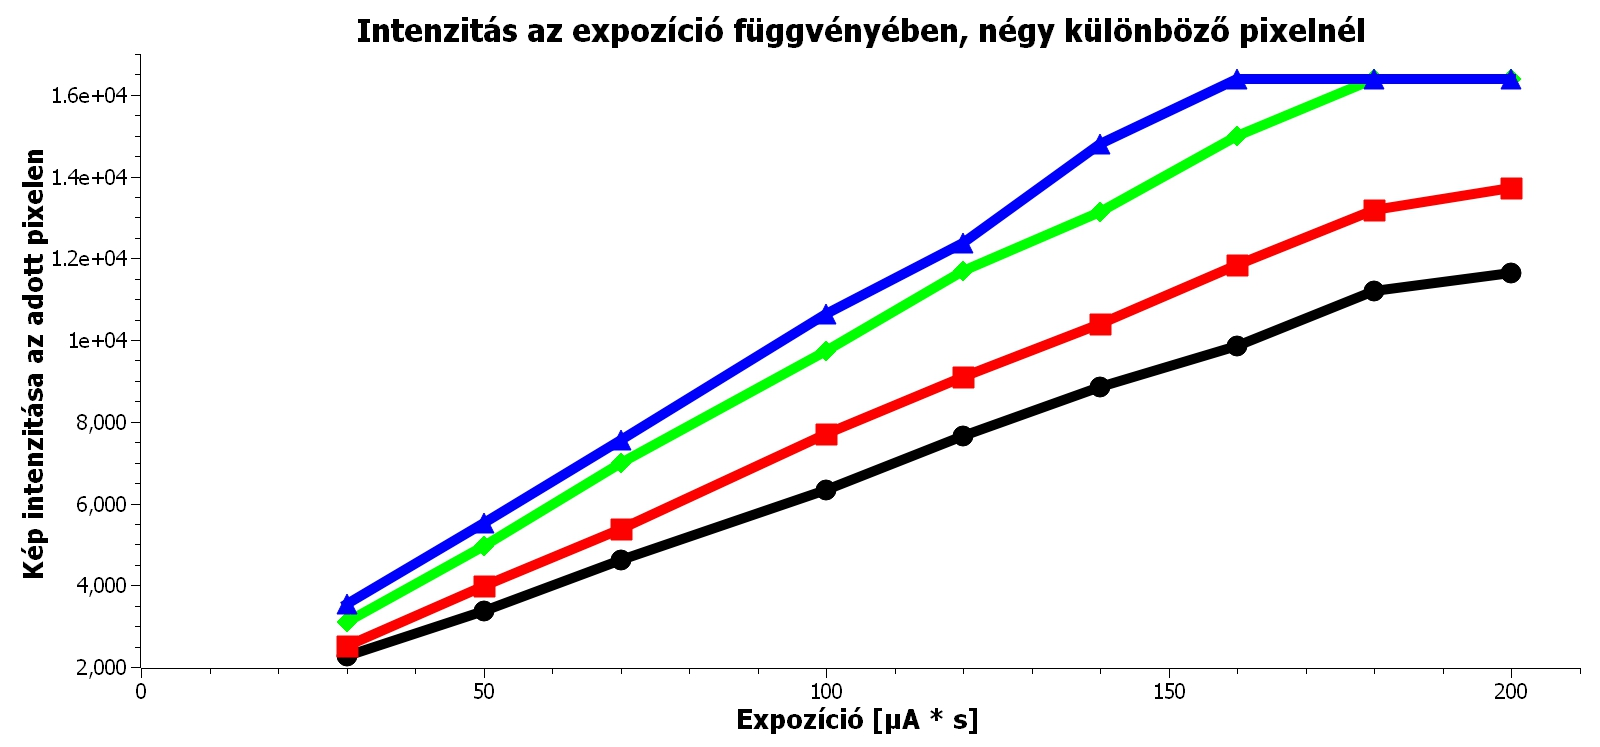
\includegraphics[width=0.8\textwidth]{abrak/gaingrafikon}
\caption{Négy kiszemelt pixel intenzitásának változása az expozíció függvényében.}
\label{fig:gaingrafikon}
\end{figure}




Az egyes hibák hatását az elkészült felvételeken \aref{fig:gainnelkul}.~ábrán szemléltetem. Az ábrán egy olyan felvétel látható, amely készítésekor a detektor és a forrás között leképezendő objektum nem volt, továbbá a felvétel mindenféle korrekciótól mentes, azaz a mérőszoftver ezt a képet olvasta ki a detektorból. Az ábrán látható, hogy a leképezendő objektum hiányában homogénnek várt kép közel sem homogén. Általánosan megfigyelhető, hogy az egyes pixelek értékei jócskán szórnak, továbbá látható, hogy a képen négyzetrácsos struktúra rajzolódik ki, amelynek oka  az, hogy detektorpanelek határainál megváltozik a pixelek érzékenysége. Különösen határozott ez az eltérés a képen látható hat függőleges egyenes mentén. Ezen pixelek az összes felvételen alacsonyabb intenzitással rendelkeznek társaiknál és értékük is kevésbé változik az expozíció növelésével, mint a többi pixel. Megfigyelhető továbbá, hogy a kép egyre sötétebb a sarkok felé, amely a flatness hibáak tudható be.

\begin{figure}[htbp]
\center
\includegraphics[width=1.0\textwidth]{abrak/gainnelkul2}
\caption{Tárgy nélkül készített felvétel, gain korrigálás nélkül.}
\label{fig:gainnelkul}
\end{figure}

A gain korrekció során tehát ezen hibákat távolítjuk el a képről. Gain korrekció után a fenti képből \aref{fig:gainnel}.~ábrán látható képet kapjuk. Megfigyelhetjük, hogy itt nem látszódnak az előbb jelölt artefaktumok. Bár a kép továbbra sem teljesen homogén -- ezt nem is várjuk el, valamekkora zaj mindenképp terhelni fogja a méréseinket --, a pixelek intenzitásának szórása jóval lecsökkent, megszűnt a gain korrekció nélküli képet átható négyzetes struktúra, és a kevésbé érzékeny pixelek sem lógnak ki a többi közül. A következőkben ezen  gain korrekcióhoz szükséges algoritmusokat ismertetem.

\begin{figure}[htbp]
\center
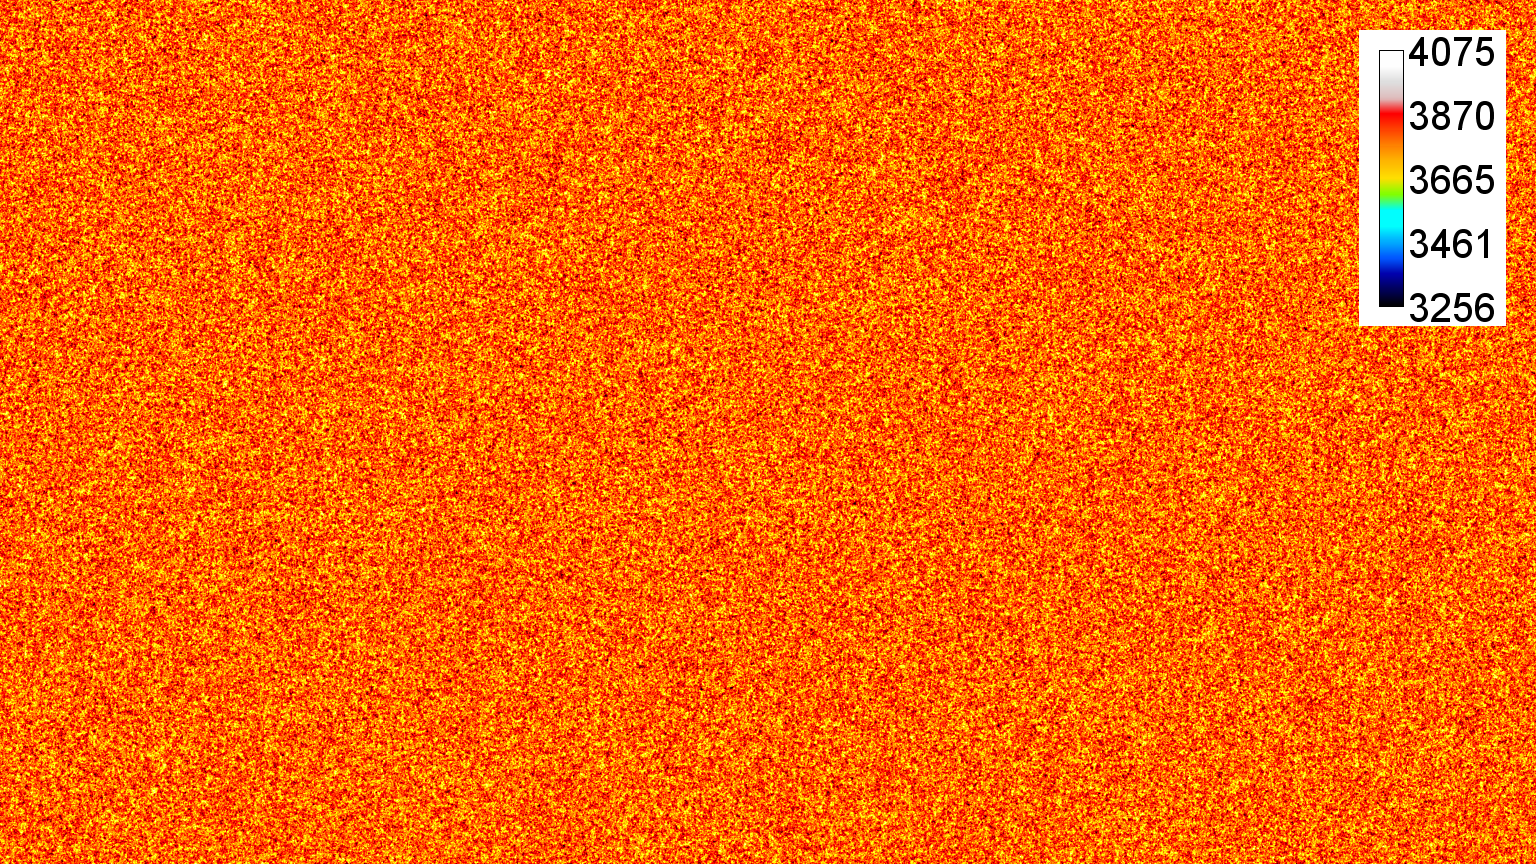
\includegraphics[width=1.0\textwidth]{abrak/gainnel}
\caption{Tárgy nélkül készített felvétel, gain korrigálás után.}
\label{fig:gainnel}
\end{figure}

\subsection{A gain korrekció algoritmusai}

A felvételek gain korrigálásához először is meg kell határozni az egyes detektorpixelekhez tartozó érzékenységeket, azaz azt, hogy az expozíció növelésével milyen gyorsan változik a pixel intenzitása, valamint azt, hogy az adott pixel milyen expozíció melett telítődik. ezen kívül meg kell határozni, hogy megvilágítás nélkül hogyan változik az adott pixel intenzitása az expozíciós idő függvényében. Ehhez először kalibráló képsorokat kell készíteni. Az offset hibák javításához a röntgenforrás bekapcsolása nélkül, különböző expozíciós időkkel, a gain és flatness hibák javításához bekapcsolt forrással, különböző expozíció értékek mellett. 

A képeket először az offset hibáktól kell megszabadítani, mivel azok a leképezendő objektumtól és a forrás beállításaitól függetlenül vannak jelen. Az ehhez szükséges korrekciós faktorok meghatározásához tehát különböző expozíciós időkkel, kikapcsolt forrással készítünk képeket. Az egyes pixelek értékét az expozíció idő függvényében ábrázolva olyan görbét kapunk, amelyre jól illeszthető egyenes. Ez alapján az $i$. pixel által, forrás nélkül mért $ I_i^{\text{offset}}$ intenzitás \aref({eq:offset}) képlettel írható le, ahol $a_i^{\text{offset}} $ és $b_i^{\text{offset}}$ a fenti módon előállított képsorozatból, egyenes illesztéssel megkapható és pixelenként változó paraméterek.

\begin{equation}
\label{eq:offset}
I_i^{\text{offset}} =  a_i^{\text{offset}} \cdot t_{\text{exp}} + b_i^{\text{offset}}
\end{equation}

Az offset hibák korrigálása után  az $i$. pixel intenzitása \aref({eq:offsetkorr})~ képlet szerint alakul, ahol $I_i^{\text{mért}}$ az $i.$ pixel eredeti, korrekció nélküli intenzitása, $I_i^{\text{offsetkorrigált}}$ pedig az offset hibától mentes érték.

\begin{equation}
\label{eq:offsetkorr}
\begin{split}
I_i^{\text{offsetkorrigált}}  &=  I_i^{\text{mért}} - I_i^{\text{offset}} \\&=  I_i^{\text{mért}} - \left( a_i^{\text{offset}} \cdot t_{\text{exp}} + b_i^{\text{offset}} \right)
\end{split}
\end{equation}


Ez után javíthatjuk ki a gain és flatness hibákat. A két hiba valójában egy algoritmussal javítható, hiszen a flatness hiba felfogható úgy, mintha a detektor pixeleinek érzékenysége lenne más a detektor más--más területein. A szükséges korrekciós faktorok meghatározásához olyan kalibráló képsorokat kell készítenünk, amelyek különböző expozícióval készülnek. \Aref{fig:gaingrafikon}.~ábrán látottak alapján megállapítható, hogy az egyes detektorpixelek intenzitása kezdetben az expozícióval lineárisan változik, vagyis egyenest tudunk rá illeszteni. Amennyiben tehát nincs tárgy a detektor és a forrás között, az $i$. pixel által, a detektort érő sugárzás, mint hasznos jel által okozott ( tehát offset hibától mentes) $ I_i^{\text{offsetkorrigált}}$  intenzitás értéke \aref({eq:gain})~egyenlet szerint számolható az expozícióból. Itt $a_i^{\text{gain}}  $ és $b_i^{\text{gain}}$ jelöli a különböző expozíciós értékek mentén felvett intenzitásértékekre illesztett egyenes paramétereit, $E$ pedig az expozíció értékét, amely a fent leírtak alapján az expozíciós idő és a röntgencső áramának szorzata.

\begin{equation}
\label{eq:gain}
\begin{split}
I_i^{\text{offsetkorrigált}}  &=  I_i^{\text{mért}} - I_i^{\text{offset}} \\&=  a_i^{\text{gain}} \cdot E + b_i^{\text{gain}}
\end{split}
\end{equation}

Egy olyan felvételen, amely készítésekor valamilyen tárgyat helyezünk a detektor és a forrás közé, a mért intenzitásértékek nyilván el fognak térni a detektor különböző részein, ahogy a leképezni kívánt tárgy lineáris gyengítési együtthatója is eltér a különböző térfogatokban. Ezt úgy vehetjük figyelembe, hogy  \aref({eq:gain})~képletben az $E$ expozíció érték helyére egy helyfüggő, $E_i^{\text{virt}}$ virtuális expozíciót vezetünk be. Ezen érték úgy módosul az eredeti $E$ expozícióhoz képest, hogy figyelembe veszi a röntgen nyaláb gyengülését, miközben az áthalad a leképezni kívánt tárgyon. Vagyis egy adott mérés során az $E_i^{\text{virt}}$ virtuális expozíció nem lesz más, mint az a (valós) expozíció érték, amely esetén ugyan akkora intenzitást mértünk volna tárgy nélküli elrendezésben, mint jelen esetben a leképezendő tárggyal. Ezzel a jelöléssel kapjuk \aref({eq:gain_virtual}) egyenletet, amely immáron általánosan igaz, egy tetszőleges felvételre -- míg \aref({eq:gain})~egyenlet csak arra az esetre érvényes, amikor nincs semmi a detektor és a forrás között.

\begin{equation}
\label{eq:gain_virtual}
\begin{split}
I_i^{\text{offsetkorrigált}}  &=  I_i^{\text{mért}} - I_i^{\text{offset}} \\&=  a_i^{\text{gain}} \cdot E_i^{\text{virt}} + b_i^{\text{gain}}
\end{split}
\end{equation}


A gain hibák javítása során azt szeretnénk elérni, hogy az egyes pixelek intenzitása ne függjön az adott pixel érzékenységétől, azaz az $a_i^{\text{gain}}  $ és $b_i^{\text{gain}}$  együtthatóktól, csak az adott pixelt ért -- virtuális -- expozíciótól. Vagyis azt, hogy ha két detektorpixelt egy felvétel során ugyanolyan intenzitású sugárzás ér, és az expozíciós idő is megegyezik, akkor a két pixel intenzitása az elkészült képen is azonos legyen. 
Ezt úgy végezzük el, hogy először meghatározzuk az egyes detektorpixelek virtuális expozícióját, majd ezekből úgy alakítjuk ki a gain korrigált intenzitásértéket, mintha minden pixel érzékenysége megegyezne.

Először tehát kiszámoljuk az adott offset korrigált intenzitáshoz tartozó virtuális expozíció értékét \aref({eq:gain_virtual})~egyenlet segítségével, amelyből egyszerű átrendezéssel kapjuk a virtuális expozícióra  \aref({eq:virtual_expozicio})~egyenletet. 

\begin{equation}
\label{eq:virtual_expozicio}
\begin{split}
 E_i^{\text{virt}} &= \frac{I_i^{\text{offsetkorrigált}} -  b_i^{\text{gain}}}{  a_i^{\text{gain}}}
 \end{split}
\end{equation}



 A virtuális expozíció tehát azzal van összefüggésben, hogy mekkora valós fluxus érte az adott pixelt, és mentes az adott pixel érzékenységek torzító hatásától. Ebből úgy határozzuk meg a gain korrigált intenzitás értéket, mintha minden pixel érzékenysége, azaz intenzitás -- virtuális expozíció függvénye egy origón átmenő egyenes lenne, mindnek azonos meredekséggel. A szóban forgó meredekséget pedig úgy határozzuk meg, hogy éppen annál az expozíciós értéknél telítődjön, amelynél a legérzékenyebb pixel már telítődik. Azaz meg kell vizsgálni, hogy az expozíciót növelve mikor kapunk olyan képet, amin már van szaturált pixel. Ezen expozíciót hívjuk szaturációs expozíciónak ($E^\text{szat}$). Ezen érték a kalibráló adatsorból szintén meghatározható paraméter. Ezen paraméter ismeretében a gain korrigált $ I_i^{\text{gainkorrigalt}}$ pixelintenzitás \aref({eq:gainkorrigalt})~egyenlettel számolható, ahol $\left(2^{14} -1\right)$ a detektor által mérhető maximális intenzitásérték.

\begin{equation}
\label{eq:gainkorrigalt}
\begin{split}
 I_i^{\text{gainkorrigalt}} &= E_i^{\text{virt}}  \cdot \frac{2^{14} -1}{E^\text{szat}}
 \end{split}
\end{equation}


A módszer hatékonyságát -- azaz azt, hogy a megfelelő adatsorokra valóban jól illeszkedik egyenes, valamint, hogy az így meghatározott korrekciós faktorokkal valóban hatékonyan lehet javítani a képek minőségét -- a kísérleti algoritmus létrehozása során Tölgyesi részletes tesztekkel vizsgálta\cite{botond}, ezért én ettől eltekintek. Ugyanakkor megjegyzem, hogy a korrekciós faktorokat külön meg kell határozni minden feszültségértékre, amin a röntgenforrást működtetjük. A feszültség módosításával ugyanis megváltozik a detektorpixelekben a sugárzás elnyelődésének valószínűsége, azaz változik a pixel érzékenysége.


A továbbiakban azt mutatom be, hogy ezeket az algoritmusokat hogyan építettem bele az elkészült szoftverbe, illetve milyen mérési utasítást ajánlok a korrekciók elkészítéséhez.


\subsection{A gain kalibráció használata}


A kalibrációs szoftver létrehozásakor szempont volt, hogy annak sebessége gyors, kezelése egyszerű legyen, így létrehoztam egy grafikus felülettel rendelkező programot, amelyben a felhasználó nyomógombokkal tud választani az elérhető funkciók között. Az első ilyen megvalósított funkció az offset és gain hibák korrigálására szolgáló együtthatók meghatározása. Ezt a funkciót választva a szoftver egy új ablakban kéri a felhasználót, hogy  válassza ki az elkészített kalibrációs mérések mappáját, valamint azt a mappát, ahova a kimeneti fájlokat menteni szeretné. Ez után a korrekciós faktorok számolása automatikusan megtörténik, minden olyan feszültségértékre, amely feszültség értékekkel megfelelő mennyiségű és minőségű kép található az adott mappastruktúrában (lásd alább). Az esetleges hibákról a felhasználó értesítést kap a konzolon.
 
 
 

A korrekciós faktorok  pixelenként kerülnek meghatározásra, így azok, mint egy együttható-térkép, képként  kerülnek mentésre.
 A diplomamunkához használt gain korrekciós faktorok 50kV-os feszültségen készült képekhez tartozó együttható térképét \aref({fig:offsetfaktorok}).~ és \aref({fig:offsetfaktorok2}).~ábrán láthatóak. A struktúrák jobb láthatósága érdekében az egyes képek ábrázolásához különböző színtérképeket használtam. Az ábrákon látjuk azt, hogy a detektor struktúrája valóban nagy hatással van az egyes pixelek érzékenységére. 
 
 
 \begin{figure}[htbp]
\center
\includegraphics[width=0.49\textwidth]{abrak/offsetslope}
\includegraphics[width=0.49\textwidth]{abrak/offsetintercept}
\caption{Offset hibák korrekciójára szolgáló együttható-térkép. Balra a korrekciós egyenes tengelymetszete, jobbra a meredeksége [ms$^{-1}$].}
\label{fig:offsetfaktorok}
\end{figure}

 
 
  \begin{figure}[htbp]
\center
\includegraphics[width=0.49\textwidth]{abrak/slope50}
\includegraphics[width=0.49\textwidth]{abrak/intercept50}
\caption{Gain és flatness hibák korrekciójára szolgáló együttható-térkép. Balra a korrekciós egyenes tengelymetszete, jobbra a meredeksége [($\mu$A $\cdot$ ms)$^{-1}$].}
\label{fig:offsetfaktorok2}
\end{figure}

 
 

 Ezekkel a korrekciós faktorokkal a felhasználónak lehetősége nyílik az elkészített projekcióit offset és gain korrigálni, az erre vonatkozó (\ref{eq:offsetkorr}) és (\ref{eq:gainkorrigalt}) képleteket felhasználva.  A felhasználónak ennél a funkciónál is grafikus felületen van lehetősége kijelölni a korrigálni kívánt mappát, amelyből a program az összes képet gain korrigálja és elmenti egy kívánt, kijelölt mappába -- akár ugyan abba. 
 
 
\subsection{A gain kalibráció implementálása és a szükséges mérések leírása} 
\label{sec:reduce}
 
 
A bemeneti fájlok elkészítéséhez, azaz a mérési utasításhoz szükséges megjegyeznem, hogy a mérések során észrevehető volt, hogy a detektor által készített képek egy része valamiért jóval sötétebb, mint az azonos körülmények között készült egyéb képek. Ez a hiba a képek kb.\ 5\%-át érinti, és okát nem sikerült felderíteni. Más felhasználók is panaszkodtak hasonló hibára ennél a detektortípusnál. A korrekciós faktorok számításánál azonban kimondottan fontos, hogy ilyen képeket ne használjunk fel a számításokhoz -- továbbá az ilyen képek kezelése egyéb helyzetekben is szükségszerűnek tűnik. Ennek érdekében a gain kalibrációhoz szükséges méréseket úgy végeztük el, hogy egy adott beállítással több képet készítettünk ( 10--20 képet beállításonként). Az azonos beállításokkal készült képeket külön mappákba mentettük, így a szoftver is ilyen formában várja azokat az adatok feldolgozása során. Ez a megoldás azért szerencsés, mert egy mappán belül átlagolva a képek intenzitásértékét, könnyen és egyértelműen kiszűrhető, ha valamelyik kép jóval sötétebb, a fent említett hiba miatt. Továbbá az azonos mappákban lévő, tehát azonos beállításokkal készült képeket átlagolva a képeket terhelő zaj is csökken. Így amikor a korrekciós faktorokat számolom, mappánként átlagolom azokat a képeket, amelyek átlagos intenzitása nem tér el 10\%-nál jobban a mappában lévő képek átlagos intenzitásának átlagától. Az program  robusztusságát  tovább növelve, a képek beolvasásakor vizsgálom, hogy  azok milyen expozíciós beállításokkal készültek, és ez alapján is szelektálom a képeket, kiszűrve a mérés során elkövetett emberi hibákat. A mérésvezérlő szoftverről ugyanis tudni érdemes, hogy a felvételek készítésének elindítása a röntgen forrás bekapcsolásától függetlenül elindítható, és az indítás után sorozatosan készít képeket, amíg le nem állítják. Mérés közben a forrás feszültsége és áramerőssége szabadon változtatható, illetve a forrás ki- és bekapcsolható. A röntgencső független kezelése részben biztonságvédelmi célokat szolgál, azonban lehetőséget ad a felhasználónak, hogy a képek sorozatos kimentését elindítsa úgy, hogy a forrás nincs bekapcsolva, vagy a beállított paraméterei nem megfelelők. Ekkor gyakran előfordul, hogy a felhasználó a paramétereket menet közben állítja, és az addigi eredményeket nem törli ki. Ezt kiküszöbölendő, a gain korrekcióhoz készített kalibrációs képek feldolgozása során a képek átlagos intenzitásán kívül a program vizsgálja az átlagos áramerősség, feszültség és exponálási idő paramétereket is, és a kilógó értékkel készült képeket figyelmen kívül hagyja. Továbbá figyelembe veszi azt is, hogy offset korrekcióhoz készült kalibráló képek között ne legyen olyan, ahol a forrás be volt kapcsolva -- vagy ha van, akkor hagyja azt is figyelmen kívül. Hasonlóan a gain és flattness hibák faktorai meghatározásánál az algoritmus ignorálja azokat a képeket, ahol a forrás ki volt kapcsolva. Amennyiben egy mappában kevés kép van, amely a fenti szűröknek megfelel (5-nél nem több), akkor a mappa tartalmát a szoftver nem használja fel a korrekciós faktorok meghatározásához. Továbbá, amennyiben túl kevés mappát talál a szoftver (5-nél nem többet), tehát túl kevés a különböző expozíciós beállítások száma a korrekciós faktorok meghatározásához -- akár összesen, akár túl kevés megy át a fenti szűrükön--, a kalibrációs  faktorok nem kerülnek meghatározásra. Így elkerülhető, hogy túl kevés pontra illesszünk egyenest, és ezért hibás eredményeket kapjunk, vagyis a képkészlet ellenőrzése szintén a szoftver robusztusságát növeli. A felvételek elkészítésekor alkalmazott feszültségértékeket az program szintén a képek beolvasásakor határozza meg, így azt külön megadni nem szükséges, mint ahogy a képeket feszültség szerint sem kell szétválogatni -- ellentétben a kísérleti algoritmussal.

A képek beolvasása és mappánkénti  átlagolása után a pixelenkénti egyenes illesztést a szokásos, egyenes illesztésére vonatkozó (\ref{eq:linearfit}) képleteket felhasználva oldottam meg, ahol az $x$ és $y$ mérési pontokra illesztjük az $\alpha$ és $\beta$ paraméterekkel jellemzett egyenest.  A képletben a felülvonás az átlagolást jelenti.

\begin{equation}
\label{eq:linearfit}
\begin{split}
\beta &= \frac{ \overline{xy} - \overline x \cdot \overline y }{\overline{x^2} - {\overline{x}}^2}\\
\alpha &= \overline y -\beta \cdot \overline x
\end{split}
\end{equation}


Jelen esetben $x$ értéke az expozíciós idő (offset hibáknál), vagy az expozíció (gain és flatness hibáknál), y pedig az adott pixel intenzitása. Az egyenes illesztésére egyszerű és gyors megoldásnak találtam, hogy az illeszteni kívánt képeket pixelemként összeadom, valamint ugyanezt megteszem az adott expozícióval -- vagy expozíciós idővel -- megszorozva is, majd ezeket a képeket pixelenként elosztom az összeadott képek számával. Így képek összeadásával és skalárral való osztásával az $\overline x$ és $\overline{xy}$ értékek pixelenként előállnak, mint egy--egy kép. Ez után a kettő különbségét -- mint képet -- leosztva az  $\left ( \overline{x^2} - {\overline{x}}^2\right )$ skalárral, közvetlenül előáll a pixelekre illesztett egyenes meredeksége, és a tengelymetszet további képkivonással kapható. Mivel a szükséges képműveletek -- összeadás, skalárral szorzás, kivonás -- könnyen párhuzamosíthatóak, gyakorlatilag az egyenes illesztése is párhuzamosan történik, így jelentősen lerövidítve a számoláshoz szükséges időt. 
%15 perc helyett 2 és fél perc. Az enyém átlagol mappánként, az övé nem.
 A módszer egyébként a memóriával is takarékosabban bánik, mint a kísérleti algoritmus, amely először beolvassa az összes képet a memóriába, majd pixelenként illeszt egyenest. Az ottani megoldással ellentétben, ahol a szükséges memória lineárisan nő a képek számával, nálam a szükséges memória a képek számától független és alacsony.


A fenti megoldáshoz a grafikus felületet és a mappakezelést a Qt biztosítja, míg a gyors képműveletek CUDA kód alkalmazásával valósulnak meg. A képfeldolgozáshoz létrehoztam olyan kép osztályt, amely képes magát fájlból a GPU memóriájába olvasni, és alkalmas a képeken végzett műveletek gyors végrehajtására a grafikus kártyán. A pixelenkénti összeadás, kivonás, skalárral szorzás megoldása viszonylag triviális, itt egy szál egy pixel értékét számolja. Ezzel ellenben a maximum, minimum és átlagos intenzitás számolása első ránézésre nem triviális, ezért néhány mondatban bemutatom. 

Az előbb felsorolt műveletek, amelyek eredménye előáll a kép pixeleiből úgy, hogy minden egyes pixel értékét egyszer használjuk fel, egy kommutatív, asszociatív, két elem között ható -- programozási értelemben vett -- operátorral, az angol irodalom  \emph{reduce} műveletnek hívja. Ilyen az előbb említett összeadás, minimum és maximum számítás is. Például három elem, $a,b$ és $c$ összegét megkapjuk, ha $a$ és $b$ összegéhez hozzáadjuk $c$-t: $\text{sum} = (a+b)+c$. Az összeadást kicserélhetjük maximum számításra is, az algoritmus ekkor csak a számok közé rakott operátorban tér el: $\text{maximum} = \text{max} ( \text{max}(a,b),c))$.  Az ilyen, \emph{reduce} típusú műveletek optimális használatát az összeadás példáján keresztül írom le, de a fentiek értelmében a minimum és a maximum számolás is hasonlóan kivitelezhető.

Az alkalmazásomban is használt reduce műveletet  a CUDA hivatalos dokumentációjához mellékelt példa \cite{reduce} alapján állítottam össze. Az ilyen műveletek általános megoldása -- az összeadás példáján --, hogy a képet két részre osztjuk, majd az egyik részt hozzáadjuk a másikhoz. A műveletet folytatjuk, mindig felezve a fennmaradó képrészletet, míg végül a kép egyik pixelében előáll az összes pixel összege. A már említett példa ezen túl olyan, CUDA specifikus technikákat is ajánl a művelet gyorsításához, mint a \emph{shared memory}, azaz az összes szál által hozzáférhető (de kívülről nem hozzáférhető), gyors elérésű memória használata -- a lassú elérésű, globális memória helyett, ahol a képek eleve tárolva vannak. Továbbá figyelembe veszi, hogy a párhuzamos futtatás során a szálak 32 darabos ,,csomagokban'',  úgynevezett \emph{warpokban} futnak, ezzel tovább optimalizálva az algoritmust. Abban az esetben ugyanis, ha több, mint 32 szálat futtatunk egyszerre, semmi nem garantálja, hogy azok egyszerre fognak futni. Ilyenkor időről időre be kell várnia a szálaknak egymást. Például ha a kép egyik felét hozzáadjuk a másikhoz, csak akkor felezhetjük tovább az elkészült képet, ha minden összeadás megtörtént. Amikor már 32-nél kevesebb szálat használunk, akkor a szálaknak nem kell egymást bevárni, hiszen biztosan nem fut több. Továbbá a példa alapján az összeadáshoz vonatkozó kerneleket C++ template-ekkel írtam meg, amely segítségével már fordítási ismertté válik, hogy adott blokkmérettel futtatva a műveletet, hol kell a képet elfelezni -- nem pedig futási időben kell $if$ műveletekkel vizsgálnia, hogy a blokk mekkora méretű. A hivatkozott példa alapján a \emph{reduce} műveletek ilyen technikákkal való megvalósítása akár $6$--$30$-szor gyorsabbak, mintha ezek nélkül valósítanánk meg a műveletet. Ez a program futási sebességére igen jótékony hatással van, hiszen a kép pixeleinek összeadására -- átlag számoláshoz -- szinte minden megnyitás után szükség van, hogy eldöntsük, hogy az az említett ismeretlen hiba miatt elsötétült e, vagy sem. 



%TODO A véletlenszerűen elsötétülő képeket itt is külön korrigálja a program: ha egy kép intenzitása jelentősen eltér a sorrendben mellette lévő képek átlagától, úgy az szoftvera képet a szomszédjainak átlagával helyettesíti a gain korigálás előtt.

\section{A geometria kalibráció}
\label{sec:geomkalib}

A diplomaunkám során a másik fő feladatom volt a  az úgynevezett \emph{geometria kalibráció} robusztus algoritmusainak megalkotása, amely segítségével a CT-vel elkészített képek alapján állapíthatjuk meg, hogy milyen távol van egymástól a detektor, a forgatható asztal forgástengelye és a röntgencső fókuszpontja. A geometriai adatokra igen pontosan szükség van, amikor az elkészült projekciók alapján meghatározzuk a felvett tárgy 3 dimenziós képét, vagyis a visszavetítéskor. Ugyanakkor a geometriai paramétereket kézzel nem tudjuk igen pontosan lemérni, már csak azért sem, mert a röntgencső fókuszpontjának a helye nem hozzáférhető és nem ismert, továbbá a mérési pontatlanság is viszonylag nagy lenne. Ezért alkalmazzuk azt a módszert, hogy a berendezéssel készített képek alapján határozzuk meg a szóban forgó paramétereket. 

A kalibrációt két cikk alapján végeztem el. Noo cikke\cite{noo} valamivel bonyolultabb  módon, kevés adatból határozza meg a geometriai paramétereket, míg Wu\cite{wu} cikke részben az előbbire támaszkodva, azonban azt leegyszerűsítve,  és több adatsorból határozza meg a távolságokat, a szerzők szerint pontosabban, mint a Noo féle megoldással. A kísérleti algoritmus ezért is csupán utóbbival dolgozik. Én azonban megvizsgáltam, hogy hibaszámítással alkalmazható e hatékonyan a Noo által leírt, kevesebb elhanyagolást tartalmazó módszer, valamint hibaszámítással javítottam a Wu által vázolt módszeren is, továbbá a kísérleti algoritmushoz képest fundamentálisan más megoldást vezettem be a képek feldolgozásához.

 A továbbiakban bemutatom a geometriai kalibráció meghatározásának elméletét a cikkek alapján, majd bemutatom, hogy a geometriai adatok meghatározásához milyen módszereket használt a kísérleti algoritmus, valamint az én algoritmusaim, továbbá ismeretem az elért eredményeimet. 

\subsection{A síkpaneles CBCT geometriája}

Hogy a geometriai kalibráció során milyen adatok kerülnek meghatározásra, és milyen adatok kerülnek elhanyagolásra, azt jól szemlélteti \aref({fig:geom1}).\ és \aref({fig:geom2}).~ábra. 



\begin{figure}[htbp]
\center
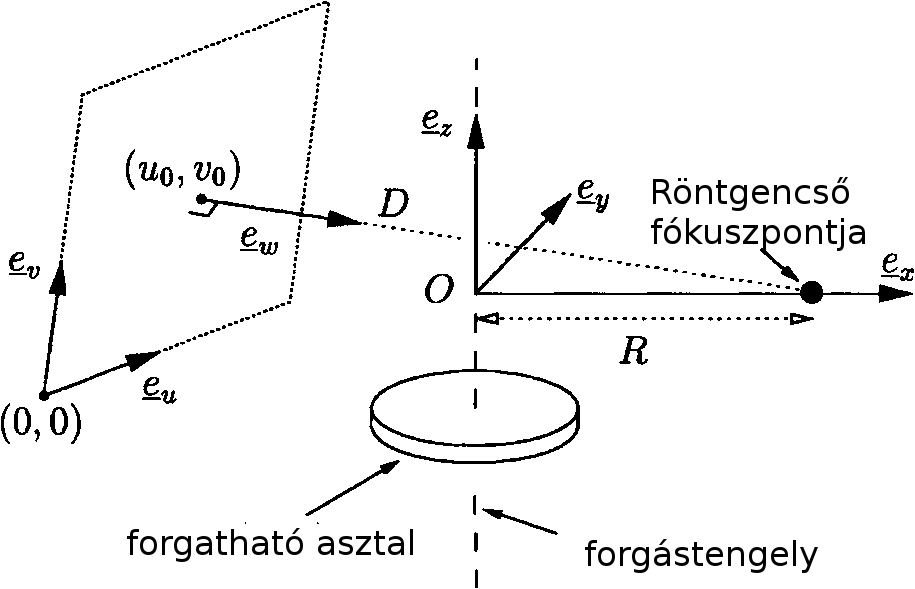
\includegraphics[width=0.5\textwidth]{abrak/geom1}
\caption{A Cone-beam CT elrendezésének vázlata\cite{noo}. A $z$ tengellyel párhuzamos forgástengely $R$ távolságra van az $x$ irányban lévő forrásponttól. A detektor és a forrás közötti legrövidebb távolság $D$. A forrásoz legközelebb eső pontja a detektornak az $u_0,v_0$ koordinátával jellemzett pixel. }
\label{fig:geom1}
\end{figure}





\Aref{fig:geom1}.~ábrán látható paraméterek jelentése a következő. A forgatható asztal forgástengelye és a röntgencső fókuszpontjának távolsága $R$. Konvenció szerint a forgástengely a $z$ tengellyel párhuzamos és az $x$ tengely irányában található a forrás fókuszpontja. A detektor az $(u_0,v_0)$ koordinátákkal jellemzett pixelétől mért távolsága a legkisebb a forrástól, és ez a távolság $D$.


\begin{figure}[htbp]
\center
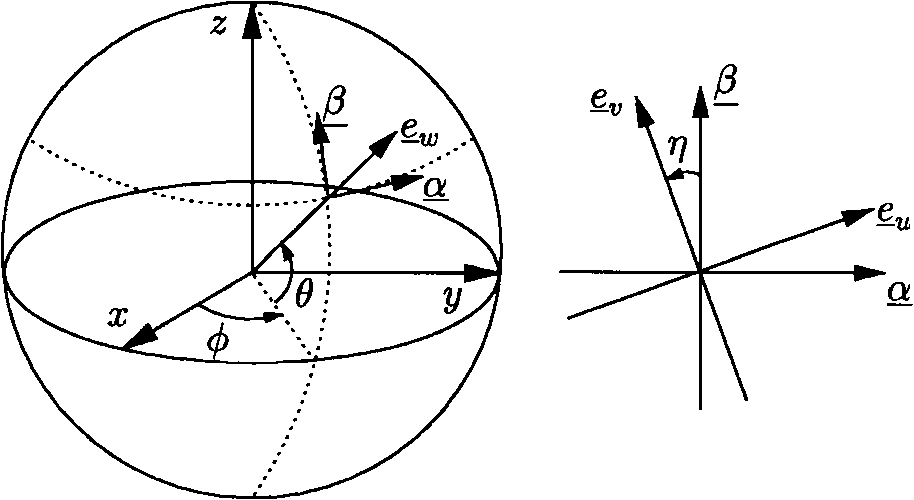
\includegraphics[width=0.5\textwidth]{abrak/geom2}
\caption{A Cone-beam CT elrendezésében jellemző irányok\cite{noo}. $\underline{e}_\omega$ a detektor síkjára merőleges irány, $\alpha$ és $\beta$ a detektor síkjában fekvő, egymásra merőleges vektorok. A detektor dőlését a $\phi, \theta,$ és $\eta$ szögek jellemzik.}
\label{fig:geom2}
\end{figure}



 \Aref{fig:geom2}.~ábrán azt láthatjuk, hogy míg a forgástengely és a forrás iránya  a modell szerint rögzített, a detektor irányát és állását a   $\phi, \theta$ és $\eta$ szögeket jellemzik. Ezek közül az $\eta$ szöget, vagyis a detektornak a saját síkjában való elfordulását mindkét cikk figyelembe veszi és számolja. A $\phi$ szöget, vagyis a detektor kifordulását, az asztal forgástengelyével párhuzamos tengely mentén, már csak Noo\cite{noo} cikke számolja ki. A $\theta$  szöggel jellemzett elfordulást pedig mindkét cikk elhanyagolja. Az elhanyagolásokra az ad lehetőséget, hogy az nem befolyásolja nagy mértékben a rekonstruált kép minőségét, illetve a többi paraméter mérési pontosságát\cite{wu}. 

 Összefoglalva tehát meghatározandó paraméter a detektor és a forrás távolsága ($D$), a forgástengely és a forrás távolsága ($R$), a detektor pixelei közül a forráshoz legközelebbi ($u_0,v_0$), valamint a detektor elfordulása a saját síkjában ($\eta$).  Ezen kívül Noo módszerével meghatározható a detektor ferdeségét jellemző $\phi$ szög is, de ez egyrészt a kísérleti algoritmusban sem került meghatározásra, másrészt az elkészült rekonstrukciós kód sem veszi figyelembe.
 

\subsection{A geometriai paraméterek meghatározásának elmélete}

A fent összegzett paraméterek az említett cikkek alapján meghatározhatóak úgy, hogy a forgatható asztalra egy plexi --  vagy egyéb, alacsony sűrűségű -- lapra fémből -- vagy egyéb, nagy sűrűségű anyagból -- készült gömb alakú tárgyakat helyezünk el, egymástól jól meghatározott távolságra, majd az asztalt körbeforgatva felvételeket készítünk. Belátható\cite{noo}, hogy a forgatás során körbeforduló gömbök a detektoron ellipszis pályát írnak le. A geometriai paramétereket ezen ellipszis pályákból tudjuk meghatározni.
Ennek módját először Noo cikke alapján mutatom be, majd ismertetem, hogy ahhoz képest Wu cikke milyen változásokat tartalmaz.

\subsubsection{A paraméterek meghatározása Noo\cite{noo} cikke alapján}
\label{sec:noo}


Az adatok feldolgozása mindkét esetben azzal kezdődik, hogy az egyes projekciókon meg kell keresni, hogy a detektoron hol jelenik meg a golyók képe. A sorrendben $k$.\ golyó helyzetét az $i$. projekción ($u_k^i, v_k^i$)-vel jelölöm. Noo cikkében két golyót tartalmazó fantomot használnak, így $k$ értéke 1 vagy 2 lehet. $i$ értéke 1 és $N$ között változik, ahol $N$ a teljes körbeforduláshoz alatt elkészített felvételek száma.  Az egyes projekción az említett koordináták megkeresése nem egyértelmű probléma, és az említett cikkek sem adnak részletes segítséget  a feladat elvégzéséhez. Így a golyók középpontjának megkeresésére nem itt, hanem a geometriai kalibráció megvalósítást tárgyaló \aref{sec:kozeppont}\ fejezetben térek ki. 

Miután a golyók középpontja az összes projekción meghatározásra került, elsőként a detektor saját síkjában való elfordulását kell korrigálni, azaz meghatározni az $\eta$ szöget. Ehhez meg kell határozni a forgástengely detektorra vetített ($\hat{u}_k, \hat{v}_k$) képét a két ellipszis esetében. \Aref{fig:etameghat}.~ábrán látható, ez a pont az épp ellentétes fázisban lévő pontok közé húzott szakaszok közös metszéspontjában van, amely nem feltétlenül esik egybe az ellipszis ($\overline{u}_k , \overline{v}_k$) középpontjával. A kereset ($\hat{u}_k, \hat{v}_k$) pont így \aref({eq:etameghat1})~egyenletrendszer alapján lineáris regresszióval kapható meg. A pontok ismeretében pedig a detektor elfordulása \aref({eq:etameghat2})~egyenlettel kapható.



\begin{figure}[htbp]
\center
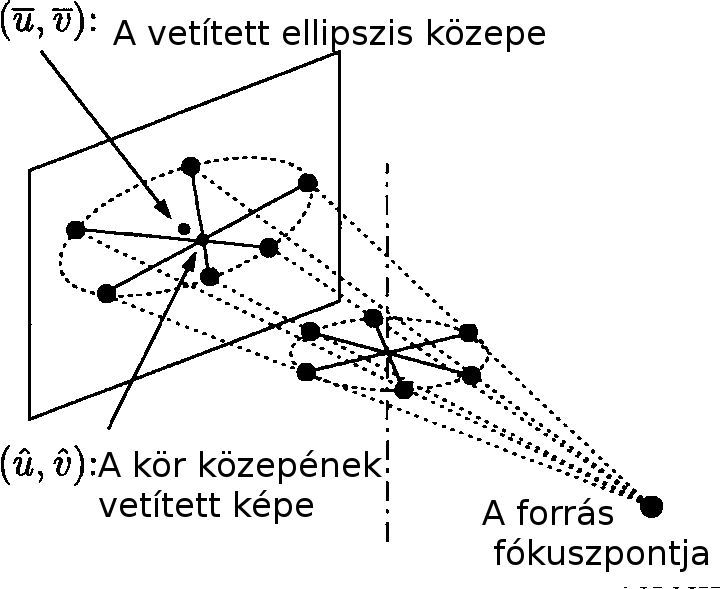
\includegraphics[width=0.5\textwidth]{abrak/etameghat}
\caption{A körbeforduló golyók vetített képe. A forgástengely vetített képe nem feltétlenül esik egybe a vetített ellipszis középpontjával.\cite{noo} }
\label{fig:etameghat}
\end{figure}


\begin{equation}
\label{eq:etameghat1}
\left(u_k^j-u_k^i \right) \hat{v}_k - \left(v_k^j-v_k^i \right) \hat{u}_k = v_k^iu_k^j - v_k^ju_k^i, \hskip10pt  j = i+ \frac{N}{2}, \hskip10pt i = 1 \ldots  \frac{N}{2} 
\end{equation}


\begin{equation}
\label{eq:etameghat2}
\eta = \arctan \left ( \frac{\hat{u}_1 - \hat{u}_2}{\hat{v}_1 - \hat{v}_2} \right )
\end{equation}



Az $\eta$ szög meghatározása után az összes projekción a golyók vetített képeinek koordinátáját el kell forgatni ezzel a szöggel. Ez után a képek úgy kezelhetőek, mintha egy ferdeségtől mentes detektorral készültek volna. Vagyis egy ellipszis ($u_k^i, v_k^i$) pontja helyett \aref({eq:forgatas})~egyenletekkel számolt (${u_k^i}^*, {v_k^i}^*$) pontot vesszük figyelembe a számolás további részében.  Csupán arra kell odafigyelni, hogy a detektoron keresett ($u_0,v_0$) koordinátákat végül vissza kell forgatni .

\begin{equation}
\label{eq:forgatas}
\begin{pmatrix}
{u_k^i}^* \\ {v_k^i}^*
\end{pmatrix}
 = 
 \begin{pmatrix}
 \cos \eta & -\sin \eta \\
 \sin \eta & \cos \eta
\end{pmatrix}
\cdot
\begin{pmatrix}
{u_k^i} \\ {v_k^i}
\end{pmatrix}
\end{equation}


Ez után az elforgatott pontokra ellipszist kell illeszteni, ahol az ellipszis pontjai \aref({eq:ellipse})~egyenletet elégítik ki. 

\begin{equation}
\label{eq:ellipse}
a \left ( {u^i}^* - \overline{u} \right )^2 + b  \left ( {v^i}^* - \overline{v} \right )^2 + 2c  \left ( {u^i}^* - \overline{u} \right ) \left ({v^i}^* - \overline{v} \right ) = 1
\end{equation}


A fenti egyenletből lineáris regresszióval meghatározhatóak az ellipszis ($\overline{u}, \overline{v}$) középpontja, az $a$ és $b$ paraméterek, amelyek a tengelyek hosszával vannak kapcsolatban, valamint $c$, amely paraméter az ellipszis ferdeségével hozható összefüggésbe.  Ezekből a paraméterekből először a forrás és a tengely távolsága ($D$) a meghatározható, \aref({eq:noo_d})~egyenletek alapján. Az újonnan meghatározott $D$ távolság ismeretében a további meghatározandó paraméterek \aref({eq:noo_tobbi})~egyenletekkel számolhatóak. Az egyenletekben $z_1$ és $z_2$ a golyók $z$ koordinátájára utal a fantomon. Amennyiben az adott golyó a fantomon a röntgenforrás vonala felett helyezkedik el, úgy előjele pozitív, amennyiben alatta, úgy előjele negatív. Ez az adat sem feltétlenül mérhető, így ezt is az elkészült felvételek alapján kell meghatározni. Továbbá \aref({eq:noo_d}).~egyenletekből az elsőnél látható $\epsilon$ tényező értéke $\pm1$: pozitív előjellel, ha a két golyó a a röntgenforrás két oldalán helyezkedik el, vagyis ha $z_1z_2 < 0$. Amikor a golyók ugyan azon az oldalon vannak, vagyis $z_1z_2>0$, akkor $\epsilon$ értéke lehet $+1$, valamint $-1$ is: ilyen esetben az előjel megállapításához szükséges a felhasználó döntése a távolság mért értéke alapján. Az egyenletekben jelen lévő $n_0, n_1, m_0, m_1, \rho_k, \zeta_k$ változók segédváltozók a többi paraméter számolásához.

\begin{equation}
\label{eq:noo_d}
\left.
\begin{split}
D^2 &= \frac{(a_1- 2n_0n_1 )- \epsilon \sqrt{a_1^2+ 4n_1^2 - 4n_0n_1a_1}}{2n1^2}\\
n_0&= \frac {1-m_0^2-m_1^2}{2m_0m_1}\\
n_1&= \frac{a_2-a_1m_1^2}{2m_0m_1}\\ 
m_0 &=\left ( \overline{v}_2 - \overline{v}_1 \right) \sqrt{b_2-\frac{c_2^2}{a_2}}\\
m_1 &= \sqrt{b_2 - \frac{c_2^2}{a_2}} \sqrt{b_1- \frac{c_1^2}{a_1}} 
\end{split}
\right\}
\end{equation}



\begin{equation}
\label{eq:noo_tobbi}
\left.
\begin{split}
v_0^* &= \overline{v}_1 - \text{sign} (z_1) \frac {\sqrt{a_1 + a_1^2D^2    }}{\sqrt{a_1b_1-c_1^2}}\\
u_0^* &= \frac{1}{2} \overline{u}_1  + \frac{1}{2} \overline{u}_2 + \frac{c_1}{2a_1} \left ( \overline{v}_1 - v_0^* \right) + \frac{c_2}{2a_2} \left (\overline{v}_2 - v_0^* \right)\\
\rho_k &= \frac{\sqrt{a_kb_k-c_k^2}}{\sqrt{a_kb_k+a_k^2b_kD^2-c_k^2}}  \hskip10pt k = 1,2\\
\zeta_k &= D \cdot \text{sign}(z_k)a_k \frac{\sqrt{a_k}}{\sqrt{a_kb_k+a_k^2b_kD^2-c_k^2}}\\
\sin \phi & = -\frac{c_1}{2a_1}  \zeta_1 - \frac{c_2}{2a_2} \zeta_2
\end{split}
\right \}
\end{equation}


Miután a fenti egyenletekkel meghatároztuk a geometriára jellemző $D, v_0^*, u_0^*$ és $\phi$ paramétereket, végül már csak a forrás és forgástengely közötti $R$ távolságot kell meghatároznunk. Ez \aref({eq:noo_r})~egyenlet lapján történik, ahol $d$ a két golyó -- valós -- távolsága a fantomon.

\begin{equation}
\label{eq:noo_r}
\begin{split}
\frac{d^2}{R^2} = \frac{1}{N} \sum_{i=1}^{N} \left\{ \left ( \zeta_1 \frac{u_1^i - u_0^*}{v_1^i - v_0^*}  - \zeta_2 \frac{u_2^i - u_0^*}{v_2^i - v_0^*} \right)^2 + \left( \frac{D \zeta_1}{v_1^i - v_0^*} - \frac{D \zeta_2}{v_2^i - v_0^*} \right)^2 + \left ( \zeta_1 - \zeta_2 \right) ^2 \right\}
\end{split}
\end{equation}


\subsubsection{A paraméterek meghatározása Wu\cite{wu} cikke alapján}
\label{sec:wu}


A fentiekhez képest a legnagyobb eltérést az jelenti Noo és Wu cikke között, hogy utóbbi esetben a fantomon nem két golyó van, hanem több, ezzel növelve a módszer megbízhatóságát. 

A paraméterek meghatározása ebben az esetben is az $\eta$ szög meghatározásával és a vele való korrekcióval történik, ám ebben az esetben -- mivel több golyó adata áll rendelkezésre -- egyenes illesztéssel tudjuk meghatározni $\tan \eta$ értékét, \aref({eq:wu_eta})~egyenlet szerint.

\begin{equation}
 \label{eq:wu_eta}
\hat{u}_k  = c + \tan \eta \cdot \hat{v}_k
\end{equation}

A mérési pontokra ez után szintén ellipszist kell illeszteni, azonban Wu cikkében \aref({eq:wu_ellipse})~egyenlet írja le a ellipszist. El van hanyagolva tehát \aref({eq:ellipse})~egyenletben még meglévő $c$ paraméter, amely akkor tehető meg, ha az ellipszis nagytengelye éppen vízszintes állású. Ez jó közelítéssel igaz is, hiszen az ellipszisen el vannak forgatva az előzetesen meghatározott $\eta$ szöggel, amely következtében a forgástengely képe a detektoron egy függőleges egyenes. Mivel az asztal körbeforgatása során a golyók merőlegesen mozognak a forgástengelyre, a vetített képükre is igaz lesz, hogy a pályájuk nagytengelye merőleges a forgástengely vetületére, azaz éppen vízszintes. 

\begin{equation}
\label{eq:wu_ellipse}
a \left ( {u^i}^* - \overline{u} \right )^2 + b  \left ( {v^i}^* - \overline{v} \right )^2  = 1
\end{equation}



Ezzel az egyszerűsítéssel a keresett geometriai paramétereket leíró egyenletek is jócskán leegyszerűsödnek. A keresett $v_0^*$ és $D$ paraméterek  \aref({eq:wu_d})~egyenletekből lineáris regresszióval megkaphatóak, amely egyelnetek a $k$ és $k'$ sorszámú ellipszisek között teremtenek kapcsolatot.

\begin{equation}
\label{eq:wu_d}
\frac{\overline{v}_k + \overline{v}_{k'}}{2}  - \frac{1}{2 \left( \overline{v}_k   - \overline{v}_{k'}  \right)} \left( \frac{1}{b_k} - \frac{1}{b_{k'}} \right) = v_0^* + D^2 \frac{1}{2 \left( \overline{v}_k   - \overline{v}_{k'} \right) }   \left( \frac{a_k}{b_k} - \frac{a_{k'}}{b_{k'}} \right)
\end{equation}

Vegyük észre, hogy Noo módszerével ellentétben itt nem szükséges a golyók függőleges pozíciójának ($z_1, z_2$) vizsgálata. Így ez a módszer minden esetben egyértelműen számolja a kérdéses paramétereket, míg Noo módszerénél az összes többi paraméter értékét meghatározó $D$ paraméter bizonyos esetekben -- amikor a kiválasztott golyók függőlegesen a forrás azonos oldalain voltak -- nem volt egyértelmű. Továbbá ez a képlet jóval egyszerűbb, mint \aref({eq:noo_d})~egyenletekben leírtak.

Ugyancsak egyszerű képletet kapunk $u_0^*$ értékére: mivel a $c$ paraméterek értékét elhanyagoljuk, a Noo által használt (\ref{eq:noo_tobbi}) képletek megfelelő sorára ránézve látszik, hogy $u_0^*$ értéke az ellipszis illesztésnél kapott $\overline{u}_k$ értékek átlagolásával kapható, vagyis  \aref({eq:wu_u0}), ahol $E$ az alkalmazott golyók -- és így az ellipszisek -- száma. 
\begin{equation}
\label{eq:wu_u0}
u_0^* = \frac{1}{E} \sum_{k=1}^E \overline{u}_k\\
\end{equation}


Ez után az egyetlen meghatározandó paraméter a forgástengely és a forrás $R$ távolsága. Ezt a távolságot most \aref({eq:wu_r})~egyenletekkel tudjuk meghatározni, amelyek egy $k$ és egy $k'$ sorszámú ellipszis között teremtenek kapcsolatot, és ahol $d^{kk'}$ a két  ellipszishez tartozó golyók távolsága a fantomon. A képletben továbbá $ \left ( \alpha_k - \alpha_{k'} \right )$ jelöli annak az elfordulásnak a szögét, amely elfordulással a két golyó az ellipszisük azonos fázisába forgathatóak. Ez a szög tehát $0^\circ$, amennyiben a golyók a plexi fantomon a forgástengely azonos oldalára vannak felerősítve, és $180^\circ$, amennyiben a fantom ellentétes oldalain vannak.

\begin{equation}
\label{eq:wu_r}
\left .
\begin{split}
\left( \frac{d^{kk'}}{R} \right) ^2 & = \left ( \zeta_k - \zeta_{k'}  \right )^2  +  \left (\rho_{k} \right )^2 + \left (\rho_{k'} \right )^2  - 2\rho_k \rho_{k'} \cos  \left ( \alpha_k - \alpha_{k'} \right ) \\
\rho_k &= \frac{1}{\sqrt{\left (\overline{v}_k - v_0^* \right)^2 \cdot b_k}}\\
\zeta_k &= \left ( \overline{v}_k  - v_0^* \right ) \frac{ 1- \left( \rho_k \right) ^2 }{D} 
\end{split}
\right\}
\end{equation}


\subsection{A geometriai kalibráló mérés kivitelezése}

A geometriai kalibrációs mérésekhez csapágygolyókat használtunk, amelyeket cellux ragasztóval rögzítettünk egy plexi lapra, \aref{fig:geomfantom}.~ábrán látható módon. Bár a megoldás nem a legprecízebb, lehetőséget ad rá, hogy a fantomot igény szerint átrendezzük. Erre akkor lehet szükség, ha például más nagyítás mellett a golyók nagy része kilógna a detektált képből.


\begin{figure}[htbp]
\center
\includegraphics[width=0.8\textwidth]{abrak/geomfantom}
\caption{A geometriai kalibrációhoz használt fantom}
\label{fig:geomfantom}
\end{figure}


 A plexin 2~mm-enkénti bemélyedés segítette a pontos pozicionálást, a golyókat ezekbe a lyukakba ragasztottuk bele. Továbbá ezen barázdarendszer a golyók távolságának leolvasását is megkönnyítette. A méréseket a lehető legmagasabb csőfeszültség mellett, 80~kV-on végeztük, a fantomot körbeforgatva. A magas feszültségre azért volt szükség, hogy a plexi minél kevésbé legyen látható az elkészült felvételeken, ezzel segítve a golyók megtalálását a képen. Ugyanakkor a magas feszültség ellenére is, amikor a lemez síkja épp párhuzamos volt a fősugárral -- tehát a detektoron \aref{fig:geomfantom}.~ábrán látható elrendezés $90^\circ$-kal való elforgatottja jelent meg, a plexi lemez a fém golyókkal összemérhető intenzitást adott, vagyis a golyók elkülönítése a plexitől ekkor nehezebb feladat, mintha a golyók intenzitása jelentősen eltérne a plexiétől. Egy ilyen helyzetben és egy 90$^\circ$-kal elforgatott helyzetben készült ábrázol \aref{fig:geomfantom_plexi}.~ábra. Láthatjuk rajta, hogy a fősugárra merőleges állásban (a felső képen) a golyók intenzitására 1000--2000 körüli érték adódik, míg a plexinél ez az érték 10~000 körüli. Elforgatott állásban a plexi és a golyók intenzitása is 1000--2000 körüli érték, vagyis ekkor már a plexi elsötétülése megegyezik a golyóékéval. Ez a a jelenség az algoritmusok tervezése során egy megoldandó problémát jelentett, amelyre \aref{sec:kozeppont}.~fejezetben térek ki. 
 
A fantomban a csapággolyók mérete változó, 






\begin{figure}[htbp]
\center
\includegraphics[width=0.8\textwidth]{abrak/geomfantom_meroleges}
\includegraphics[width=0.8\textwidth]{abrak/geomfantom_parhuzamos}
\caption{A geometriai kalibrációhoz használt fantom}
\label{fig:geomfantom_plexi}
\end{figure}







\subsection{A geometriai kalibráció megvalósítása}



A geometriai kalibráció robusztus algoritmusainak megalkotása során rendelkezésemre állt a kísérleti algoritmus során eredményesnek bizonyult megvalósítás\cite{botond}, ami lényegében \acite{wu} cikken alapult,  valamint felhasználtam  \acite{noo} cikkben leírtakat is. Míg utóbbi csak két golyó adataival dolgozik, kevesebb elhanyagolást alkalmaz. Előbbi azonban egyszerűbb képleteket használ, eleve több golyós fantomot feltételezve, amely gyakran lineáris regresszióvá alakítja a képleteket, felhasználva egyszerre az összes golyó adatait. Mindkét cikk algoritmusát implementáltam a programomban, megvizsgáltam, hogy vajon a kevesebb elhanyagolást eredményező változat robusztussá tehető e, ha a több golyó adatait megfelelő hibaszámítással súlyozva átlagolom. A hibaszámítást a másik algoritmus megvalósítása során is bevezettem, így mindkét módszernél kezelem az esetleges hibákat a golyók keresése és az ellipszisek illesztése során. Továbbá új algoritmust vezettem be a golyók középpontjának megkeresésére, amely a felhasználótól kevesebb információt kér, pontosabban eredményt ad,, valamint a videókártyán való megvalósításnak köszönhetően hamar lefut.

A következőkben bemutatom a geometriai korrekciós faktorok meghatározásának folyamatát az elkészült programban, ismertetem a  megtervezett algoritmusokat és azok használatának lehetőségeit és korlátait, valamint az eredményeit.


\subsubsection{ A folyamat áttekintése és a felhasználótól kért adatok. }


Az általam megvalósított kalibrációs szoftver újabb funkciója a geometriai korrekciós mérések kiértékelése. A funkció kiválasztásakor először beolvasásra kerülnek a gain kalibráció adatai, amely helyének kiválasztására a felhasználónak grafikus felületen van lehetősége. Szintén grafikus felületen választható ki az, hogy hol keresse a program a geometriai kalibrációhoz szükséges képkészletet. A mappában lévő képek ezek után egy csúszka mozgatásával átnézhetőek, továbbá szintén grafikus felületen várja a program a szükséges felhasználótól bekérendő adatok megadását. Ezek az adatok a következők:

\begin{itemize}
  \item Első felhasználni kívánt kép sorszáma.
  \item Azon golyók száma, amelyek az összes képen rajta vannak.
  \item Azon golyók száma, amik nincsenek rajta az összes képen.
  \item Az első képpel azonos állású, $360^\circ$-kal elforgatott kép sorszáma.
  \item A forrás és a detektor becsült távolsága mm-ben.
    \item A fantomon a golyók egymástól vett távolságát.
\end{itemize}

Az első kép kiválasztására azért van lehetőség, mert a felhasználó hibázhat a mérés elindításakor: nem kapcsolja be a röntgen forrást, nem indíja el a motort, stb... A keresendő golyók száma szintén fontos, a golyók keresésénél felhasznált paraméter. Az általam megvalósított algoritmusnak segítséget ad az is, hogy tudja, hogy bizonyos képeken több golyó lehet a képen, mint az elsőn -- például mert a kép alsó és felső szélén lévő golyók vetülete a detektoron kívülre eset és így a képről eltűnhet a forgatás hatására. Ennek megállapításához a felhasználónak eleve át kell néznie azon képeket, amik egy teljes körbefordulás alatt készültek, így arra is megkéri a program, hogy a csúszkát ez után hagyja egy olyan állapotban, amely nagyjából  $360^\circ$-kal van elforgatva az első képhez képest. Itt nem szükséges pontosan a teljes körbeforduláshoz tartozó projekciót megadni, a felhasználó ettől eltérhet $\pm 45^\circ$-kal. A cél itt az, hogy a felhasználó jelölje ki, körül-belül hol kell keresni a teljes körbefordulást, hogy annak megkeresése rövidebb időt vegyen igénybe, mintha az összes projekciót át kellene nézni. Szükséges továbbá a Noo féle számításhoz megadni a detektor és a forrás távolságát. Erre azért van szükség, mert ahogy \aref{sec:noo} fejezetben említettem, a Noo féle módszernél ezen távolság kiszámítása azon esetekben, amikor a két kiszemelt golyó a forgástengely azonos oldalán vannak, nem egyértelmű. Ennek eldöntését segíti a felhasználó által megadott paraméter, amely szintén nagyságrendi becslést kell, hogy adjon, tehát pár centiméteres hiba még megengedett. Ez után egy újabb grafikus felületen kell megadni a fantomon a golyók helyzetét, amelyből a távolságuk kiszámításra kerülnek.


Amennyiben ez megtörtént, a felhasználó ellenőrizheti, hogy az algoritmus jó helyen találta e meg a golyókat a kezdeti képen, illetve, hogy a teljes körbefordulás utáni kép egyezik e az elsőnek választottal. Amennyiben bármelyikben hibázott a program, lehetőség van visszalépni, és újabb kezdeti projekciót választani. A grafikus felület egy ilyen állapotát mutatja meg  \aref{fig:geomui}.~ábra. 


\begin{figure}[htbp]
\center
\includegraphics[width=0.8\textwidth]{abrak/geomui}
\caption{A geometriai kalibrációs funkció felhasználói felülete. A felhasználó a fenti mappát választotta ki a képek helyéül. A bal oldali képet választotta első képnek, az alsó részen pedig megadta a szükséges paramétereket. A szoftver meghatározta a teljes körbefordulás utáni projekciót és megkereste a két projekción a gömbök középpontját. }
\label{fig:geomui}
\end{figure}



A kijelölt projekció módosítására egyébként a diplomamunkám elkészítése során nem kellett sort kerítenem, az első képen is biztosan felismerte a golyók helyzetét a program és a körbefordulás utáni képet is stabilan megtalálta. Az esetleges hibás felismerések elkerülése végett ugyanakkor érdemes olyan projekcióról indítani a kalibrációt, amelyen a plexi elsötétedése alacsony mértékű.


A kísérleti algoritmusnál megvalósítottakhoz  képest ez a felület jóval felhasználóbarátabb, kevesebb információt kér a felhasználótól, kisebb a felhasználó hibázási lehetősége is -- ahol a program számot vár, ott szöveget nem tud megadni, stb.

A program a felhasználó jóváhagyása után az alább ismertetett algoritmusokkal kiszámolja a kalibrációs faktorokat, majd az eredményt közli a felhasználóval. A folyamat  jó részét a képek feldolgozása, azaz a golyók középpontjának megkeresése teszi ki. A feldolgozás állapotáról a felhasználó egy folyamatjelző sávon tudja követni.






\subsubsection{Teljes körbefordulás meghatározása}

A szoftver első feladata, még a felhasználótól való adatbekérés során, hogy meghatározza, melyik projekció felel meg az elsőként kiválasztott projekció $360^\circ$-kal való elforgatottjának. Ehhez a felhasználó megad egy viszonyítási alapot: egy olyan képet, amely nagyjából megfelel a fenti kritériumnak. A szoftver ez után a két kép sorszámának különbségét elosztja $8$-cal. A teljes körbefordulás képét a felhasználó által megadott kép körül ilyen távolságban keresi, a képek sorszámainak tekintetében. Így nem kell megvizsgálni a teljes mappa tartalmát, csupán annak egy részét, amely következtében a körbefordult kép megkeresése kevesebb időt vesz igénybe. 


A teljes körbefordulást vizsgálatot úgy végzem, hogy az első képpel korrerálom a kiválasztott második képpel, és megvizsgálom, hogy a korreláció melyik kép választása esetén a legnagyobb. Ez a kép lesz a teljes körbefordulás utáninak választott kép. A kiválasztott $A$ és $B$ közötti kép $C$ korrelációs együtthatóját \aref({eq:corr})~képlet alapján végzem, ahol az összegzés a kép összes pixelére vonatkozik, a felülvonás az átlagolást jelenti, $\sigma$ pedig a képek szórását jelöli. A műveletet grafikus kártyán, párhuzamosan végzem. Az átlagokat és a szórásokat pedig a művelet előtt, szintén grafikus kártyán párhuzamosítva végzem: az átlagoláshoz a pixelek értékeit össze kell adni, a szórás pedig a pixel értékeinek négyzetösszegéből származtatható. Így valójában mindkét művelet \aref{sec:reduce} fejezetben bemutatott, könnyne párhuzamosítható \emph{reduce} műveletet testesíti meg.

\begin{equation}
\label{eq:corr}
C = \frac{ \sum_{i=1}^{N}  \left \{ (A_i  - \overline{A} ) \cdot ( B_i - \overline{B} ) \right \} }{N \cdot \sigma_A  \cdot \sigma_B}
\end{equation}


A fenti módon számolt korrelációs érték $0$ és $1$ közötti értéket vehet fel: a kép önmagával való korrelációs együtthatója éppen $1$. Ez alapján a szoftver vizsgálhatja azt is, hogy a megtalált kép eléggé hasonlít e az elsőként kiválasztott képre. Amennyiben a korrelációs együttható $0,\!9$ alatt van, vagyis az elsőként kijelölt képhez talált legnagyobb korrelációjú párja sem hasonlít eléggé az eredetire, a szoftver figyelmezteti a felhasználót.



\subsubsection{A golyók középpontjának meghatározása}
\label{sec:kozeppont}



Amennyiben a felhasználó minden adatot megadott, megkezdődik a képek feldolgozása, amelynek során először meghatározásra kerülnek az egyes projekciókon a golyók koordinátái. Tölgyesi\cite{botond} munkája során erre két algoritmust implementált. Az egyiknél a kép kis részleteinek egy körlap képével való korrelációját számolja. Ez a módszer bizonytalannak bizonyult és ezért már a korábbi munka során el lett vetve. A másik módszere szerint a képeket először invertálja ( hogy a nagy elnyelésű golyók helyén a kép intenzitása nagy legyen), majd golyók helyét a kép egy részletén belül az ott látható képpontok intenzitással súlyozott súlypontjába becsüli.  Ennek az algoritmusnak is van hátulütője. Egyrészt megfelelő méretű ablakot kell választani, hogy a golyó épp beleessen a vizsgált tartományba és ennek az ablaknak a helyét minden projekciónál számon kell tartani. Kifejezetten hibás eredményhez vezethet ez az algoritmus akkor, amikor a golyókat épp a fősugárral párhuzamosan álló plexi lapon próbáljuk megtalálni. Ekkor a plexi lap okozta gyengülés \aref{fig:geomfantom_plexi}.~ábrán látottak alapján összemérhető, vagy akár nagyobb, mint a golyó által okozott. A plexi ilyenkor jelentős mértékben befolyásolni tudja a súlypontkeresést, akár téves útra térítve a golyók keresését. Ez ellen a vizsgált ablak csökkentésével lehet, de teljesen nem kiküszöbölhető.

A fenti hibák elkerülése érdekében a körök középpontjainak megkereséséhez egy új fajta  algoritmust használtam fel: a Hough-transzformációt. Ez az igen széles körben használt módszer  körök, egyenesek, illetve akár tetszőleges alakzatok lokalizálására használható. Körök keresése esetében először a képeken található éleket kell megkeresni, vagyis a képen található körök szélén lévő pixeleket. Majd a képre olyan körvonalakat kell rajzolni -- ezeket a továbbiakban másodlagos köröknek nevezem --, amely koröknek középpontjai az eredeti körvonalról kerülnek kiválasztásra. Amennyiben a keresett kör sugara ismert, a másodlagos  köröket is ilyen sugárral kell megrajzolunk. Ekkor a rajzolt körök közös metszete adja meg a keresett, eredeti kör középpontját. Egy ilyen eljárást szemléltet  \aref{fig:houghcircles}.~ábra. Az ábrán lévő piros kör középpontját úgy találjuk meg, hogy a körvonal kijelölt pontjaiból újabb köröket rajzolunk -- az ábrán fekete színnel. A legtöbb másodlagos kör által érintett -- kék -- pont adja meg a keresett kör középpontját. Természetesen érdemes a keresett kör összes pontja -- vagyis a képen az összes él-pont -- köré másodlagos köröket rajzolni, hogy minél pontosabb eredményt kapjunk. A módszer használható akkor is, ha a keresett kör sugara nem ismert. Ekkor ugyan azon pontokból különböző sugárral húzunk másodlagos körvonalakat. Mivel az eredeti körnek csak a középpontja van egyenlő távolságra a körvonal pontjaitól, a különböző sugarú másodlagos körök csak akkor fogják egymást egy pontban metszeni, ha a sugaruk éppen a keresett kör sugarával egyezik meg. Vagyis ismeretlen sugarú kör keresése esetén több féle sugárral kell másodlagos köröket rajzolni, és meg kell keresni, hogy  melyik sugár alkalmazása esetén metszi egymást a legtöbb kör. Ekkor megtaláltuk a keresett kör sugarát, a metszések helye pedig megadja a keresett kör középpontját.

\begin{figure}[htbp]
\center
\includegraphics[width=0.49\textwidth]{abrak/houghcircles}
\caption{Körkeresés Hough-transzformációval.}
\label{fig:houghcircles}
\end{figure}




A Hough-transzformációval tehát kimondottan  kör alakú objektumokat tudunk a képen keresni, és emellett az algoritmus jól párhuzamosítható is, hiszen az élkeresés egy konvolúciós művelettel elvégezhető, amely után a képre az él pixelek közepéből húzott körvonalak szintén párhuzamosan rajzolhatóak. A továbbiakban bemutatom, hogy a körkeresést pontosan hogyan implementáltam az elkészült programban.


A körkeresés  első lépés tehát az élek megkeresése. Erre több algoritmus is használható. Először a képet simítani szükséges, hogy az esetleges zajok ne befolyásolják az élkeresést. Ez után kerülnek kiválasztásra az él-pixelek, amelyre  két gyakori megoldás a következő.

\begin{itemize}
\item Kiszámoljuk a kép gradiensét, azaz azt, hogy egy adott pontban milyen gyorsan változik a kép intenzitása. A nagy intenzitásváltozású helyek jelölik ki az éleket.

\item Hattatjuk a képre a Laplace-operátort, vagyis kiszámoljuk a kép második deriváltját. Ott jelöljük ki az éleket, ahol a kép Laplace-ának  értéke előjelet vált, vagyis ahol szélsőértéke van a gradiensnek.

\end{itemize}

Előbbi jóval egyszerűbben számolható, hiszen a gradiens képen az adott pixel értéke eldönti, hogy él-pixel e vagy sem, hiszen csak azt kell vizsgálni, hogy értéke a kijelölt küszöbérték feletti, vagy sem. Az utóbbi módszernél vizsgálni kell az egyes pixelek környezetét, hogy kiderüljön, hogy az adott helyen a kép Laplace-a előjelet vált e. Vagyis ez a módszer számításigényesebb, ugyanakkor biztosabb eredményt ad.

A helyes algoritmus megválasztása során annak minőségét tartottam szem előtt, a futási sebességgel szemben, így végül a számításigényesebb, Laplace értékekkel való  élkeresést választottam. Ugyanis amikor a legkisebb csapágygolyó épp a plexi takarásában van, a gradiens módszer nem bizonyult hatékonynak. Ekkor ez a módszer nem tudta megkülönböztetni a golyó éleit a plexi élétől. Ezt \aref{fig:kisgolyo1}.~ábrán szemléltetem. A bal oldali ábrán a golyó képét láthatjuk, jobb oldalon pedig a sárga vonallal kijelölt szakasz mentén vett intenzitásértékek grafikonját. A golyó helyén, azaz a szakasz $10--20$ pixelei között az intenzitásértékek alig változnak.    \Aref{fig:kisgolyo2}.~ábrán, amelyen ugyanannak a felvételnek a gradiens képe látható, észrevehetjük, hogy a felső golyó körvonala mentén a gradiens érték valóban nem kiemelkedően magas a plexi lemez határán mérhetőhöz képest, míg a nagyobb golyók határainál jóval magasabb gradiens érték figyelhető meg.  

\begin{figure}[htbp]
\center
\includegraphics[width=0.49\textwidth]{abrak/kisgolyo}
\includegraphics[width=0.49\textwidth]{abrak/kisgolyo_intenzitas}
\caption{A plexi takarásában lévő legkisebb golyó képe, valamint az intenzitás értékek változása a golyó vízszintes metszetében -- a bal oldali képen sárga egyenessel kijelölve.}
\label{fig:kisgolyo1}
\end{figure}


\begin{figure}[htbp]
\center
\includegraphics[width=0.49\textwidth]{abrak/gradiens_kisgolyo}
\caption{A plexi takarásában lévő és más golyók, a kép gradiensén.}
\label{fig:kisgolyo2}
\end{figure}

Gradiens alapon tehát nem sikerül jól elválasztani a golyól szélét a plexi lemez szélétől, ami a Hough-transzformáció során rossz eredményeket produkálhat, ugyanis így  a plexi szélében lévő kisebb görbületek miatt a keresett kis csapágygolyó közepén lévő Hough-transzformált érték gyakran alulmúlja a plexi lemez miatt máshol megjelenő értékeket. Így ezen speciális esetekben a Hough-transzformált nem a golyó középpontjánál lesz a legmagasabb értékű.


A gradiens módszer helyett ezért a Laplace-operátorral kapott kép null-átmenetei alapján választottam ki az él-pixeleket. Ez alapján a végül megvalósított algoritmus a következőképp alakult. A felvételeket gain korrigálás után egy $\sigma = 1,\!4$ paraméterű, Gauss-eloszlású mátrixszal konvolválva elmostam a zajok kiszűrése érdekében, valamint meghatároztam a kép Laplace-át . A két műveletet egyszerre lehet elvégezni, hiszen a konvolúció tulajdonságai alapján elég a képet egy olyan mátrix-szal konvolválni, amely a Gauss-eloszlású mátrix Laplapce-operátort szimbolizáló mátrix-ával konvolválva kapjuk meg.  Tehát a mátrix elemeit a Gauss-görbe második deriváltjából kell mintavételezni, amely függvényt \aref({eq:LoG})~egyenlet írja le. Az egyenletben, és a továbbiakban az angol irodalomban használatos \emph{LoG} jelölést használtam a Gauss görbével simított kép Laplace-ának jelölésére, $\sigma$ pedig a Gauss görbe szórása. Az egyenletből egy $9x9$ méretű mátrixot alkottam meg, mint a \emph{LoG} művelet konvolúciós mátrixát. Az elkészült mátrix grafikusan ábrázolva \aref{fig:logkernel}.~ábrán látható.

\begin{equation}
\label{eq:LoG}
\text{LoG} = \frac{-1}{\pi \sigma^2} \cdot \left ( 1-\frac{x^2+y^2}{2\sigma^2} \right ) \cdot e^{-\frac{x^2+y^2}{2\sigma^2}}
\end{equation}

\begin{figure}[htbp]
\center
\includegraphics[width=0.49\textwidth]{abrak/logkernel}
\caption{$\sigma = 1,\!4$ paraméterű Gauss görbe Laplace-a.}
\label{fig:logkernel}
\end{figure}


Az élkeresésnél a gain korrigált felvételeket ezzel a mátrix-szal konvolválva kaptam meg a simított kép Laplace-át, amelyen ez után a nullátmenetek helyét kerestem meg. Ennél a lépésnél minden pixelre megvizsgáltam, hogy az adott pixel függőleges, illetve vízszintes szomszédjainak előjele eltér e. Továbbá bevezettem egy újabb kritériumot is az  élpixelek keresésénél, mégpedig azt, hogy a szomszédos pixeleknek ne csak az előjele térjen el, hanem a nulla átmenet legyen elég erős, azaz az átmenet olyan ellentétes előjelű értékek között valósuljon meg, amelyek abszolút értéke nagyobb, mint egy kritikus érték. Ezt a kritikus értéket a \emph{LoG} művelettel kapott kép szórásának a felének határoztam meg. Az ilyen módon meghatározott él-pixelek nagy része a golyók határát jelölte ki, mégpedig úgy, hogy a kisebb golyók szélének a nagy részét is megtalálta az algoritmus. Az eddigi felvételen személtetve ez a módszer\aref{fig:242_circles}.~ábra bal oldali képén feltüntetett pixeleket találja meg élként. Ha a gradiens módszerrel szeretnénk olyan élképet kapni, amely a felső, kis méretű golyó kerületének jó részén felismeri az éleket, akkor olyan küszöbértéket kel választani a gradiens képen, amellyel a jobb oldali képén látható pixeleket kapjuk éleknek. Vegyük észre, hogy a gradiens módszer jelentős mennyiségű pixelt észlel élnek ott, ahol a plexi határa található, és a kép hátterében is zajos képet ad. Ezek a tényezők rontják a Hough-transzformált minőségét és növelik a futási idejét. Az eredeti képet jobban elmosva, azaz nagyobb szórású Gauss görbével konvolválva kaphatnánk ennél kevésbé zajos él-képet a gradiens módszerrel is, de ekkor azt tapasztaltam, hogy a kisebb golyók éle is kevésbé válik felismerhetővé az él-képen. 


\begin{figure}[htbp]
\center
\includegraphics[width=0.33\textwidth]{abrak/242_zerocross_vagott}
\includegraphics[width=0.33\textwidth]{abrak/0242_gradienttreshold}
\caption{Élpixelek a szoftverben megvalósított módon Laplace-transzformálttal (balra), valamint gradiens küszöböléssel (jobbra).}
\label{fig:242_circles}
\end{figure}


A gradiens alapú élkeresést tehát elvetettem, és a Laplace alapú algoritmussal állítottam elő az él-képet. Ezt ezután Hough-transzformáltam. Mivel a felvételeken a körök sugara nem ismert, és projekciónként és mérésenként is változóak, a Hough-transzformációt a következőképp valósítottam meg.Az él-pixelek köré különböző sugarú köröket rajzolok, vagyis az eredeti képpel megegyező méretű képeket készítetek, ahol a pixelek intenzitása helyett most a pixelek azt a számot tárolják, hogy hány, adott sugarú másodlagos kör metszi egymást azon a helyen. Ezeket a képeket a továbbiakban másodlagos képeknek nevezem. Több féle sugárral megrajzolva a másodlagos köröket, a kapott másodlagos képekből úgy alakítottam ki a végső Hough-transzformált képét, hogy minden pixelnek a másodlagos képeken felvett legnagyobb értékét adtam végső értékül. Vagyis a végső Hough-transzformált képen ($HT$) az $i$ pixel értéke az $r$ sugarú másodlagos körök rajzolatából kapott $HT^r_i$ képekből \aref({eq:hough})~egyenlet alapján keletkezik. A másodlagos képeket $r_{min} = 5$ és $r_{max}=25$ közötti sugarú körök rajzolásával készítettem, de ez a paraméter igény esetén könnyedén átállítható.


\begin{equation}
\label{eq:hough}
\text{HT}_i^{vegso} = \max_{r_{min}<=r<=r_{max}} \left(HT^r_i \right)
\end{equation}


Az így kapott Hough-transzformált kép egy részlete \aref{fig:242_hough}.~ábra bal oldalán látható. A képen a maximális intenzitásokat megkeresve meghatározhatóak a körök középpontjai. A megtalált középpontokat az eredeti képen piros kereszttel jelölve a jobb oldali ábrán tüntettem fel. Jól látszik, hogy a köröket igen pontosan megtalálta az algoritmus.

\begin{figure}[htbp]
\center
\includegraphics[width=0.417\textwidth]{abrak/242_max_cropped2}
\includegraphics[width=0.33\textwidth]{abrak/0242_korok}
\caption{A kép Hough-transzformáltja (balra) és a megtalált körök középpontjai az eredeti felvételen jelölve (jobbra).}
\label{fig:242_hough}
\end{figure}


A középpontok kereséséhez használt összes képtranszformációt grafikus kártyán valósítottam meg, így azok párhuzamosan futva, gyorsan dolgozzák fel a képeket. A feldolgozás során kiszűrésre kerülnek az egyes projekción a transzformált kép maximum értékeinek helyei. Szám szerint annyi ilyen pont kerül meghatározásra, amennyit a felhasználó előzetesen megadott, beleértve azon golyók számát is, amiket a felhasználó megjelölt, mint a felvételek valamelyikén a detektor látóteréből kilépő golyó. Így a felvételek azon részén, ahol nem esik minden golyó képe a detektorra,  olyan pixeleket is azonosíthat az algoritmus golyó középpontnak, ahol valójában nincs is golyó. Ez a képek feldolgozását nem zavarja, ugyanis az egyes ellipszisekhez tartozó koordinátákat a következőképp gyűjtöm össze. A felhasználó által kijelölt első projekción meghatározásra kerülnek azon golyók középpontjai, amelyek azon a képen láthatóak. Így fontos kérés a felhasználó felé, hogy kezdetben olyan képet adjon meg, amelyen nincs olyan golyó, amely bármikor is eltűnik a detektorról. Ezen golyók középpontjai -- amelyet a felhasználó a további feldolgozás előtt ellenőriz és jóváhagy -- mellé fogja gyűjteni a szoftver az ellipszispálya további pontjait, úgy, hogy minden projekcióról választ egy pontot, mint az adott ellipszishez tartozó pont. Alapvetően a Hough-transzformált képen található  maximális intenzitású pixeleket rendeli a szoftver az egyes ellipszisekhez, úgy, hogy egy adott ellipszis adatsorához az előző projekción megtalált pixelhez legközelebb eső Hough-maximumot rendeli. Amennyiben valamely ellipszis adatsorához olyan pozíciót rendelnénk, amely az előzőtől jócskán eltér -- önkényesen megadva:  függőlegesen több, mint $15$ pixellel, illetve vízszintesen több, mint $100$ pixellel --, úgy az előző projekción meghatározott pozíció közvetlen környezetéből választok koordinátát az adott ellipszishez, aszerint, hogy az adott környezetben az új képen hol a legnagyobb a Hough-transzformált értéke. Ilyen eset akkor fordulhat elő, ha valamiért nem sikerült megtalálni egy golyót az adott felvételen. Az eljárás meggátolja a szoftvert, hogy ilyenkor túlságosan kiszóró pontot adjon hozzá valamelyik ellipszis koordináta-halmazához.




\subsubsection{Ellipszis illesztés}


Az egyes ellipszisekhez tartozó adatsorokhoz meg kell határozni a rájuk illeszthető ellipszis paramétereit. Ezt \acite{noo} cikk alapján úgy végeztem el, hogy az egyes ellipszisekhez kerestem azon $p_0,p_1,p_2,p_3,p_4$ együtthatókat, amelyekkel \aref({eq:ellipsefit})~egyenletrendszer bal oldala a legkisebb négyzetes eltérést eredményezi a jobb oldalhoz képest. 

\begin{equation}
\label{eq:ellipsefit}
p_0 (u^i)^2 - 2p_1u^i - 2p_2v^i + 2p_3u^iv^i + p_4 = -(v^i)^2 \hskip10pt i=1..N
\end{equation}

A legkisebb négyzetek probléma megoldását a CUDA \emph{cusolverSpScsrlsqvqrHost} függvényével állítottam elő. Ezen paraméterekből az  a további feldolgozás szempontjából lényeges, (\ref{eq:ellipse})~egyenletben bevezetett $a,b,c,\overline{u},\overline{v}$ együtthatókat \aref({eq:ellipsefitparameters}) egyenletekkel lehet megkapni. Bár a paraméterek meghatározása a két vizsgált cikkben eltérő módon van megvalósítva, az ellipszis illesztést a fent leírtak szerint, Noo\cite[noo] cikke alapján végeztem el. A Wu\cite{wu} cikkben leírtak alapján csak az ellipszis $c$ paramétere van elhanyagolva, amely igen jó közelítéssel már a fenti illesztésből is következik. 


\begin{equation}
\label{eq:ellipsefitparameters}
\left .
\begin{split}
\overline{u} &= \frac{p_1-p_2p_3}{p_0-p_3^2}\\
\overline{v} &= \frac{p_0p_2-p_1p_3}{p_0-p_3^2}\\
a &= \frac{p0}{p_0\overline{u}^2 + \overline{v}^2 + 2p_3\overline{u} \overline{v} - p_4} \\
b &= \frac{a}{p_0}\\
c &=p_3b
\end{split}
\right  \}
\end{equation}


A paraméterek kiszámolásán túl kiszámoltam azok hibáját is. Ehhez \acite{ellipse} forrást használtam fel, amely alapján a fenti egyenlettel definiált ellipszis adott $p_i$ paraméterének hibáját \aref({eq:ellipsefiterror})~képlettel lehet becsülni, ahol $N$ a teljes körbefordulás során felvett projekciók száma, $z_{ij}$ pedig \aref({eq:ellipsefitparameters})~egyenlet alapján
 a $p_i$.\ paraméterhez tartozó geometriai érték: $p_0$ esetén $\left(u^i\right)^2$, stb. A kifejezés számlálójában így az illesztés során kapott négyzetes eltérés látható, míg a nevezőben az illesztett paraméterhez tartozó geometriai adatok négyzete, szorozva a rendszer szabadsági fokaival, ami $5$ paraméter keresése esetén az összes adatsor számánál $5$-tel kisebb.


\begin{equation}
\label{eq:ellipsefiterror}
\sqrt{\frac{\sum_{j=1}^N \left ( \sum_{i=0}^4 p_i z_{ij} + \left (v^j \right)^2 \right)^2 }{(N-5) \sum_{j=1}^N z_{ij} ^2 }}
\end{equation}


\subsubsection{A geometriai paraméterek számítása}

Az illesztett ellipszis  $a,b,c,\overline{u},\overline{v}$ paraméterei alapján a geometriai paramétereket  \aref{sec:noo} és \aref{sec:wu} fejezetben bemutatott képletek segítségével számoltam.

Először kiszámításra kerül a detektor ferdeségét jellemző $\eta$ paraméter. A két cikk hasonló módszerrel számolja ezt, az egyetlen különbség, hogy Wu cikke elve több golyóval számol, így egyenest illeszt a tengely vetített képeire. Épp ezért a számítások során az $\eta$ paramétert egyféleképpen, egyenes illesztéssel határoztam meg. A $k$. golyó forgástengelyének vetített  $\hat{u}_k, \hat{v}_k$ koordinátáit \aref({eq:etameghat1}) képlet szerint lineáris regresszióval határoztam meg, szintén a CUDA \emph{cusolverSpScsrlsqvqrHost} függvényével. Mivel az egyes koordináták hibája nem ismert, itt az illesztés négyzetes hibájával tudom jellemezni a kapott  $\hat{u}_k, \hat{v}_k$  paraméterek jóságát, amit a továbbiakban $\hat{\sigma}_k$-val jelölök.  Ezen paraméterek segítségével $\tan \eta$ értékét a hibával terhelt mérésekre vonatkozó egyenes illesztés képleteivel számolom. Általános esetben az egyenletek az $y=a\cdot x + b$ egyenletű egyenes $a,b$ paramétereit határozzák meg az $x_i,y_i$ mért pontokból, ahol $\sigma_i$ az $y_i$ paraméter hibája. A keresett paraméterek és hibáik \aref({eq:illeszteshibaval1})~jelöléseket használva \aref({eq:illeszteshibaval2})~egyenletek alapján történhet. 


\begin{equation}
\label{eq:illeszteshibaval1}
\left .
\begin{split}
S = \sum \frac{1}{\sigma_i^2}, \hskip10pt S_x = \sum \frac{x_i}{\sigma_i^2}, \hskip10pt S_y = \sum \frac{y_i}{\sigma_i^2} \\
 S_{xx} = \sum \frac{x_i^2}{\sigma_i^2}, \hskip10pt S_{xy} = \frac{x_iy_i}{\sigma_i^2}, \hskip10pt \Delta = S\cdot S_{xx}  - \left(S_x \right) ^2
 \end{split}
 \right \}
\end{equation}

\begin{equation}
\label{eq:illeszteshibaval2}
\left .
\begin{split}
a&=\frac{S_{xx} \cdot S_y - S_x \cdot S_xy }{\Delta}\\
b&=\frac{S\cdot S_{xy} - S_x \cdot S_y}{\Delta}\\
\sigma_a^2 & = \frac{S_{xx}}{\Delta },  \hskip10pt \sigma_b^2 = \frac{S}{\Delta}
\end{split}
\right \}
\end{equation}


Bár a fenti módszer matematikailag csak abban az esetben korrekt, ha  csak az  $y_i$ paramétereket terheli a $\sigma_i$ hiba, jelen esetben  a módszer fizikailag releváns eredményt ad, hiszen valójában az egyes mérési pontok súlyozása történik a mért hiba inverzének négyzetével. A képletekben $x,y$ és $\sigma$ helyére az $\hat{u}_k, \hat{v}_k$ és $\hat{\sigma}_k$ értékeket helyettesítve az illesztett egyenes meredeksége megadja $\tan \eta$ értékét, annak hibájával együtt. Ebből számolom a program futása során az $\eta$ paramétert, annak hibájával együtt. Minthogy mind az $\eta$ szög, mind annak hibája igen kicsi érték ( $\approx 1\pm 0\!,1$ fok), a hibát a további számolás során elhanyagolom, azt csupán a felhasználó számára írom ki. Az $\eta$ paramétert pedig felhasználom arra, hogy a mért koordinátákat a detektor ferdeségével korrigáljam, azaz elforgassam azokat.


A további paramétereket a program a két cikk alapján külön --külön számolja. 

Noo metódusa szerint a fennmaradó paraméterek egy--egy ellipszis ($v_0^*$), illetve egy--egy ellipszis pár ($D, u_0^*, \phi, R$) alapján határozhatók meg.  Mindegyik paraméter esetében úgy jártam el, hogy kiszámoltam a paraméter értékét az adott ellipszisre vagy ellipszispárra, valamint kiszámoltam a paraméter hibáját is, az ellipszis illesztése során meghatározott hibák alapján kvadratikus hibaterjedéssel. Majd a geometriai paraméter végső értékét úgy számoltam ki, hogy az egyes részeredményeket azok hibájának inverzének négyzetével súlyoztam, és átlagoltam az értékeket. Ellipszispárok esetében a párok alapján számolt részeredmények közötti korrelációt nem vettem figyelembe a számítások során, mindenhol az összes ellipszispárból számolt eredményeket átlagoltam, a hibájuk alapján súlyozva.

Wu metódusa eleve több ellipszist feltételez, így például D és $v_0^*$ értékét is egyenes illesztéssel határozza meg, ahogy azt \aref({eq:wu_d})~egyenlet leírja. Itt szintén az $\eta$ meghatározása során használt módszert alkalmaztam, azaz a hibával terhelt mérésekre vonatkozó (\ref{eq:illeszteshibaval1}) és (\ref{eq:illeszteshibaval2}) egyenletek alapján illesztettem egyenest. Az illesztés során figyelembe vett hibát \aref({eq:wu_d})~egyenlet függő változójának (bal oldal) hibájával becssültem.  Mivel $u_0^*$ ennél a módszernél az illesztett $\overline{u}_k$ paraméterek átlagolásával történik, a hibaszámítással figyelembe vett, hiba inverzének négyzetével való súlyozással kapott átlag itt teljesen korrekt módszerként használtam. A Wu módszer egyetlen ellipszispáronként számolt paramétere  \Aref({eq:wu_r}) egyenlet alapján számolt $R$ paraméter, vagyis a forrás és a forgástengely távolsága. Itt szintén ellipszis páronként határoztam meg az $R$ értéket és az adott ellipszispárra kapott hiba négyzetének inverzével súlyozva  kaptam a paraméter becslését az összes ellipszis adatainak felhasználásával. 


A geometriai paraméterek számolása során tehát mindvégig számoltam a paraméterek hibáját, és a végső paraméterek számolásához az összes ellipszis adatát felhasználva kaptam meg. A kísérleti algoritmusban az átlagolás az ellipszispárokra súlyozás nélkül történt, én azonban a köztes paraméterek hibáját felhasználva, az alapján súlyozva határoztam meg a keresett geometriai paramétereket. Így amennyiben valamely ellipszis pontjai pontatlanul kerülnek meghatározásra, az a végeredményt nem torzítja el, hiszen ez esetben az ellipszis illesztésekor annak paraméterei nagy hibával kerülnek meghatározásra, így az adott ellipszis kis súllyal fogja befolyásolni a kimeneti paramétereket. A szoftver tehát felhasználói beavatkozás nélkül figyelembe veszi az adatsorok jóságát és azok alapján számítja ki a geometriai adatokat.


\section{Eredmények}



A teljes körbefordulás alatt összegyűjtött koordináták közül két ellipszishez tartozót ábrázoltam \aref{fig:ellipses}.~ábrán. Az ábrákon fekete színnel láthatóak azok a koordináták, amelyeket az én algoritmusom határozott meg. Piros színnel látható a kísérleti algoritmus által meghatározott koordináták, ugyan azon projekciókból. Bár az én algoritmusom csak egész koordinátákban tudja meghatározni az egyes projekciókon a golyók középpontját, a jóval pontosabb alakzatfelismerés miatt ez nem ront az adatsor minőségén. Az ábrákon látható, hogy az általam használt módszer kevesebb kiszóró pontot eredményez, és a kiszórás mértéke is alacsonyabb, mint a kísérleti algoritmusban megvalósított módszernél. A felső képnél alsó részén például láthatjuk, hogy a pálya középén, épp akkor, amikor a plexi lap jelentős elsötétedést okoz a képen, a kísérleti algoritmus által meghatározott koordináták jelentősen eltérnek a valódi pályától. Az alsó képen, amelyen egy sokkal kisebb kistengelyű ellipszis látható, észrevehetjük, hogy a kísérleti algoritmus által kiolvasott koordináták bár nem egész számok, hibájuk nagyobb, mint $1$ pixel: a adatsort egy periodikus ingadozás terheli, a jobb szélen jelentős mennyiségű kiszóró ponttal. 


\begin{figure}[htbp]
\center
\includegraphics[width=0.9\textwidth]{abrak/ellipse1}
\includegraphics[width=0.9\textwidth]{abrak/ellipse2}
\caption{Teljes körbefordulás alatt meghatározott golyó középpontok, két ellipszis mentén. Fekete színnel ábrázolva az általam implementált algoritmus által meghatározott koordinátákat, piros színnel a kísérleti algoritmus által meghatározott koordinátákat.}
\label{fig:ellipses}
\end{figure}






%
%
%
%\begin{table}[]
%\centering
%\label{tab:logkernel}
%\begin{tabular}{|c|c|c|c|c|c|c|c|c|}
%\hline
%0.0046  & 0.0034  & 0.0013  & -0.0008 & -0.0016 & -0.0008 & 0.0013  & 0.0034  & 0.0046  \\ \hline
%0.0034  & 0       & -0.0048 & -0.009  & -0.0107 & -0.009  & -0.0048 & 0       & 0.0034  \\ \hline
%0.0013  & -0.0048 & -0.0126 & -0.0193 & -0.022  & -0.0193 & -0.0126 & -0.0048 & 0.0013  \\ \hline
%-0.0008 & -0.009  & -0.0193 & -0.0281 & -0.0316 & -0.0281 & -0.0193 & -0.009  & -0.0008 \\ \hline
%-0.0016 & -0.0107 & -0.022  & -0.0316 & -0.0354 & -0.0316 & -0.022  & -0.0107 & -0.0016 \\ \hline 
%-0.0008 & -0.009  & -0.0193 & -0.0281 & -0.0316 & -0.0281 & -0.0193 & -0.009  & -0.0008 \\ \hline
%0.0013  & -0.0048 & -0.0126 & -0.0193 & -0.022  & -0.0193 & -0.0126 & -0.0048 & 0.0013  \\ \hline
%0.0034  & 0       & -0.0048 & -0.009  & -0.0107 & -0.009  & -0.0048 & 0       & 0.0034  \\ \hline
%0.0046  & 0.0034  & 0.0013  & -0.0008 & -0.0016 & -0.0008 & 0.0013  & 0.0034  & 0.0046  \\\hline
%\end{tabular}
%\caption{ $\sigma$  = 1.4 paraméterű Gauss függvény Laplace-transzformáltja.  }
%\end{table}




\clearpage

%\begin{thebibliography}{9}

\bibliographystyle{huplain}
\bibliography{bibfile} 


%
%\bibitem{reduce}
%Mark Harris,
%{\it Optimizing Parallel Reduction in CUDA},
%{\tt online: http://docs.nvidia.com/cuda/samples/6\_Advanced/reduction/doc/reduction.pdf},
%Utolsó hozzáférés: 2016.05.28. 14:00
%
%\bibitem{Noo}
%Frédéric Noo, Rolf Clackdoyle, Catherine Mennessier, Timothy A White, Timothy J Roney,
% {,,Analytic method based on identification of ellipse parameters for scanner calibration in cone-beam tomography},
% \emph{Physics in Medicine and Biology},
% vol. 45,
%  number={11},
%  pages={3489},
%  url={http://stacks.iop.org/0031-9155/45/i=11/a=327},
%  year={2000},
%  abstract={This paper is about calibration of cone-beam (CB) scanners for both x-ray computed tomography and single-photon emission computed tomography. Scanner calibration refers here to the estimation of a set of parameters which fully describe the geometry of data acquisition. Such parameters are needed for the tomographic reconstruction step. The discussion is limited to the usual case where the cone vertex and planar detector move along a circular path relative to the object. It is also assumed that the detector does not have spatial distortions. We propose a new method which requires a small set of measurements of a simple calibration object consisting of two spherical objects, that can be considered as `point' objects. This object traces two ellipses on the detector and from the parametric description of these ellipses, the calibration geometry can be determined analytically using explicit formulae. The method is robust and easy to implement. However, it is not fully general as it is assumed that the detector is parallel to the rotation axis of the scanner. Implementation details are given for an experimental x-ray CB scanner.}
%}
	
%\bibitem{url}
%{\tt http://fizipedia.bme.hu/index.php/Gamma\_spektroszkópia},
%2013.~november~29., 1:00

%\bibitem {nagy}
%Nagy L. Gy.,
%{\it Radiokémia és izotóptechnika},
%Tankönyvkiadó, Budapest, 1983.
%\bibitem {lederer}
%C.M. Lederer, J.M. Hollander, I. Perlman,
%{\it \foreignlanguage{english}{Table of Isotopes}},
%Wiley, New York, 1984.
%\end{thebibliography}
\end{document}